%%%%%%%% ICML 2022 EXAMPLE LATEX SUBMISSION FILE %%%%%%%%%%%%%%%%%

\documentclass[nohyperref]{article}

% Recommended, but optional, packages for figures and better typesetting:
\usepackage{microtype}
\usepackage{graphicx}
\usepackage{subfigure}
\usepackage{booktabs} % for professional tables
\usepackage{float}
% hyperref makes hyperlinks in the resulting PDF.
% If your build breaks (sometimes temporarily if a hyperlink spans a page)
% please comment out the following usepackage line and replace
% \usepackage{icml2022} with \usepackage[nohyperref]{icml2022} above.
\usepackage{hyperref}
\usepackage{array,multirow}
	
 \usepackage{xcolor}
\usepackage{color, colortbl}
\definecolor{LightGray}{gray}{0.9}
\definecolor{Gray}{gray}{0.85}
\usepackage{makecell}
\renewcommand\theadalign{bc}
% \renewcommand\theadfont{\bfseries}

\newcommand{\modky}[1] {\textcolor{blue}{#1}} 
\newcommand{\modyj}[1] {\textcolor{red}{#1}} 
\newcommand{\add}[1] {\textcolor{blue}{#1}} % for revision

\newcommand\blfootnote[1]{%
  \begingroup
  \renewcommand\thefootnote{}\footnote{#1}%
  \addtocounter{footnote}{-1}%
  \endgroup
}

% Attempt to make hyperref and algorithmic work together better:
\newcommand{\theHalgorithm}{\arabic{algorithm}}
\usepackage[ruled, vlined, linesnumbered]{algorithm2e}


% Use the following line for the initial blind version submitted for review:
\usepackage{icml2023}

% If accepted, instead use the following line for the camera-ready submission:
% \usepackage[accepted]{icml2022}

% For theorems and such
\usepackage{amsmath}
\usepackage{amssymb}
\usepackage{mathtools}
\usepackage{amsthm}

\newcommand{\bs}{\boldsymbol}
\usepackage{amssymb}% http://ctan.org/pkg/amssymb
\usepackage{pifont}% http://ctan.org/pkg/pifont
\usepackage{accents} 
\newcommand{\cmark}{\ding{51}}%
\newcommand{\xmark}{\ding{55}}%
\newcommand{\asty}{\accentset{\ast}{\mathbf{Y}}}
\newcommand{\gty}{\mbf{Y}^{\text{gt}}}
\newcommand{\mc}{\mathcal}
\newcommand{\mbf}{\mathbf}
% if you use cleveref..
\usepackage[capitalize,noabbrev]{cleveref}

%%%%%%%%%%%%%%%%%%%%%%%%%%%%%%%%
% THEOREMS
%%%%%%%%%%%%%%%%%%%%%%%%%%%%%%%%
\theoremstyle{plain}
\newtheorem{theorem}{Theorem}[section]
\newtheorem{proposition}[theorem]{Proposition}
\newtheorem{lemma}[theorem]{Lemma}
\newtheorem{corollary}[theorem]{Corollary}
\theoremstyle{definition}
\newtheorem{definition}[theorem]{Definition}
\newtheorem{assumption}[theorem]{Assumption}
\theoremstyle{remark}
\newtheorem{remark}[theorem]{Remark}

% Todonotes is useful during development; simply uncomment the next line
%    and comment out the line below the next line to turn off comments
%\usepackage[disable,textsize=tiny]{todonotes}
\usepackage[textsize=tiny]{todonotes}

% The \icmltitle you define below is probably too long as a header.
% Therefore, a short form for the running title is supplied here:
\icmltitlerunning{ZegOT: Zero-shot Segmentation Through Optimal Transport of Text Prompts}

\begin{document}

\twocolumn[
\icmltitle{ZegOT: Zero-shot Segmentation Through Optimal Transport of Text Prompts}




%%%%%%%%%%%%%%%%%%%%%%%%%%%%%%%%%%%%%%%%%%%%%%%%%%%%%%%%%%%%%%%%%%%%%%%%%%%%%%%
%%%%%%%%%%%%%%%%%%%%%%%%%%%%%%%%%%%%%%%%%%%%%%%%%%%%%%%%%%%%%%%%%%%%%%%%%%%%%%%
% Affiliation

\icmlsetsymbol{equal}{*}

\begin{icmlauthorlist}
\icmlauthor{Kwanyoung Kim}{equal,yyy}
\icmlauthor{Yujin Oh}{equal,yyy}
\icmlauthor{Jong Chul Ye}{yyy}
\end{icmlauthorlist}

\icmlaffiliation{yyy}{School of AI, Korea Advanced Institute of Science and Technology (KAIST), Daejeon, Republic of Korea}

\icmlcorrespondingauthor{Jong Chul Ye}{jong.ye@kaist.ac.kr}

% You may provide any keywords that you
% find helpful for describing your paper; these are used to populate
% the "keywords" metadata in the PDF but will not be shown in the document
\icmlkeywords{Machine Learning, ICML}

\vskip 0.3in
]


%\printAffiliationsAndNotice{}  % leave blank if no need to mention equal contribution
\printAffiliationsAndNotice{\icmlEqualContribution} % otherwise use the standard text.





%%%%%%%%%%%%%%%%%%%%%%%%%%%%%%%%%%%%%%%%%%%%%%%%%%%%%%%%%%%%%%%%%%%%%%%%%%%%%%%
%%%%%%%%%%%%%%%%%%%%%%%%%%%%%%%%%%%%%%%%%%%%%%%%%%%%%%%%%%%%%%%%%%%%%%%%%%%%%%%
\begin{abstract}

% The paper abstract should begin in the left column, 0.4~inches below the final
% address. The heading `Abstract' should be centered, bold, and in 11~point type.
% The abstract body should use 10~point type, with a vertical spacing of
% 11~points, and should be indented 0.25~inches more than normal on left-hand and
% right-hand margins. Insert 0.4~inches of blank space after the body. Keep your
% abstract brief and self-contained, limiting it to one paragraph and roughly 4--6
% sentences. Gross violations will require correction at the camera-ready phase.


Recent success of large-scale Contrastive Language-Image Pre-training (CLIP) has led to great promise in zero-shot semantic segmentation by transferring image-text aligned knowledge to  pixel-level classification. 
However, existing methods usually require an additional image encoder or retraining/tuning the CLIP
module.
Here, we present a cost-effective strategy using text-prompt learning that keeps the entire CLIP module frozen while fully leveraging its rich information. 
Specifically,  we propose a novel \textbf{Z}ero-shot s\textbf{eg}mentation with \textbf{O}ptimal \textbf{T}ransport (ZegOT) % model  
method that matches multiple text prompts with frozen image embeddings through optimal transport, which allows each text prompt to efficiently focus on specific semantic attributes. 
%Also, ZegOT deeply aligns the text prompts with intermediate layers of the frozen image encoder, which significantly boosts the zero-shot segmentation performance. 
Additionally, we propose Deep Local Feature Alignment (DLFA) that deeply aligns the text prompts with intermediate local feature of the frozen image encoder layers, which significantly boosts the zero-shot segmentation performance.
Through extensive experiments on benchmark datasets, we show that our method achieves the state-of-the-art (SOTA) performance with only $\times$7 lighter parameters compared to previous SOTA approaches. 
%% 아래는 넣어야할지 고민 -> 빼야될듯
%Moreover, the proposed ZegOT successfully closes the performance gap between seen and unseen class segmentation, which suggests that our simple but effective method can be a great solution for various zero-shot dense prediction tasks.

%Recently, the success of classification with a large-scale visual language model such as CLIP led to research into transferring knowledge from the image level to the pixel level.
%However, the general ideas almost rely on CLIP’s classification capability, resulting in a two-stage scheme that requires an additional image encoder. Due to the inevitable structure, it results in high computational cost and memory complexity. 
%To address this issue, we propose a light-efficient one-stage paradigm that generalizes the CLIP’s zero-shot capability from image-text to pixel-text score maps with at least parameters.
%First, we propose a simple-effective baseline that aligns visual embeddings and text embeddings at all of the layers by using FPN. It leads to significantly boosting performance. 
%Secondly, instead of learning only one prompt, we propose to learn multiple prompts to focus on specific attributes or contexts for each prompt.
%Finally, we optimize the optimal transport distance to align visual feature and multiple prompts through the Sinkhorn algorithm, which efficiently align the cross-modality without further learning.
%Through extensive experiments on three benchmarks, our proposed method achieved state-of-the-art results in a “transductive” setting. In addition, our method only requires $\times$20 fewer learnable parameters compared with the two-stage method, and even $\times$5 compared to the other one-stage method.
%Through extensive experiments on three benchmarks, our proposed method achieved state-of-the-art results in a “transductive” setting. 
\end{abstract}






%%%%%%%%%%%%%%%%%%%%%%%%%%%%%%%%%%%%%%%%%%%%%%%%%%%%%%%%%%%%%%%%%%%%%%%%%%%%%%%
%%%%%%%%%%%%%%%%%%%%%%%%%%%%%%%%%%%%%%%%%%%%%%%%%%%%%%%%%%%%%%%%%%%%%%%%%%%%%%%
\section{Introduction}
\label{submission}



Zero-shot Semantic Segmentation (ZS3) is one of label-efficient %deep learning methods
approach for dense prediction task, which reduce efforts for expensive pixel-level annotations of unseen object categories \cite{bucher2019zero}.
Vision language models (VLM) such as CLIP \cite{radford2021clip} have brought great advance in  ZS3 task by transferring pre-trained image-text aligned knowledge to 
%image pixel-level 
{pixel-text level} category matching problems \cite{ding2022zegformer, xu2021zsseg, zhou2022maskclip, rao2022denseclip, zhou2022zegclip}.  
The key idea here is to use the VLM knowledge gained through contrastive learning on large-scale image-text pairs through a special knowledge transfer process tailored to ZS3.




%%%%%%%%%%%%%%%%%%%%%%%%%%%%%%%%%%%%%%%%%%%%%%%%%%%%%%%%%%%%%%%%%%%%%%%%%%%%%%%
%% Front Comparison Figure

\begin{figure}[!t]
\vskip 0.1in
\begin{center}
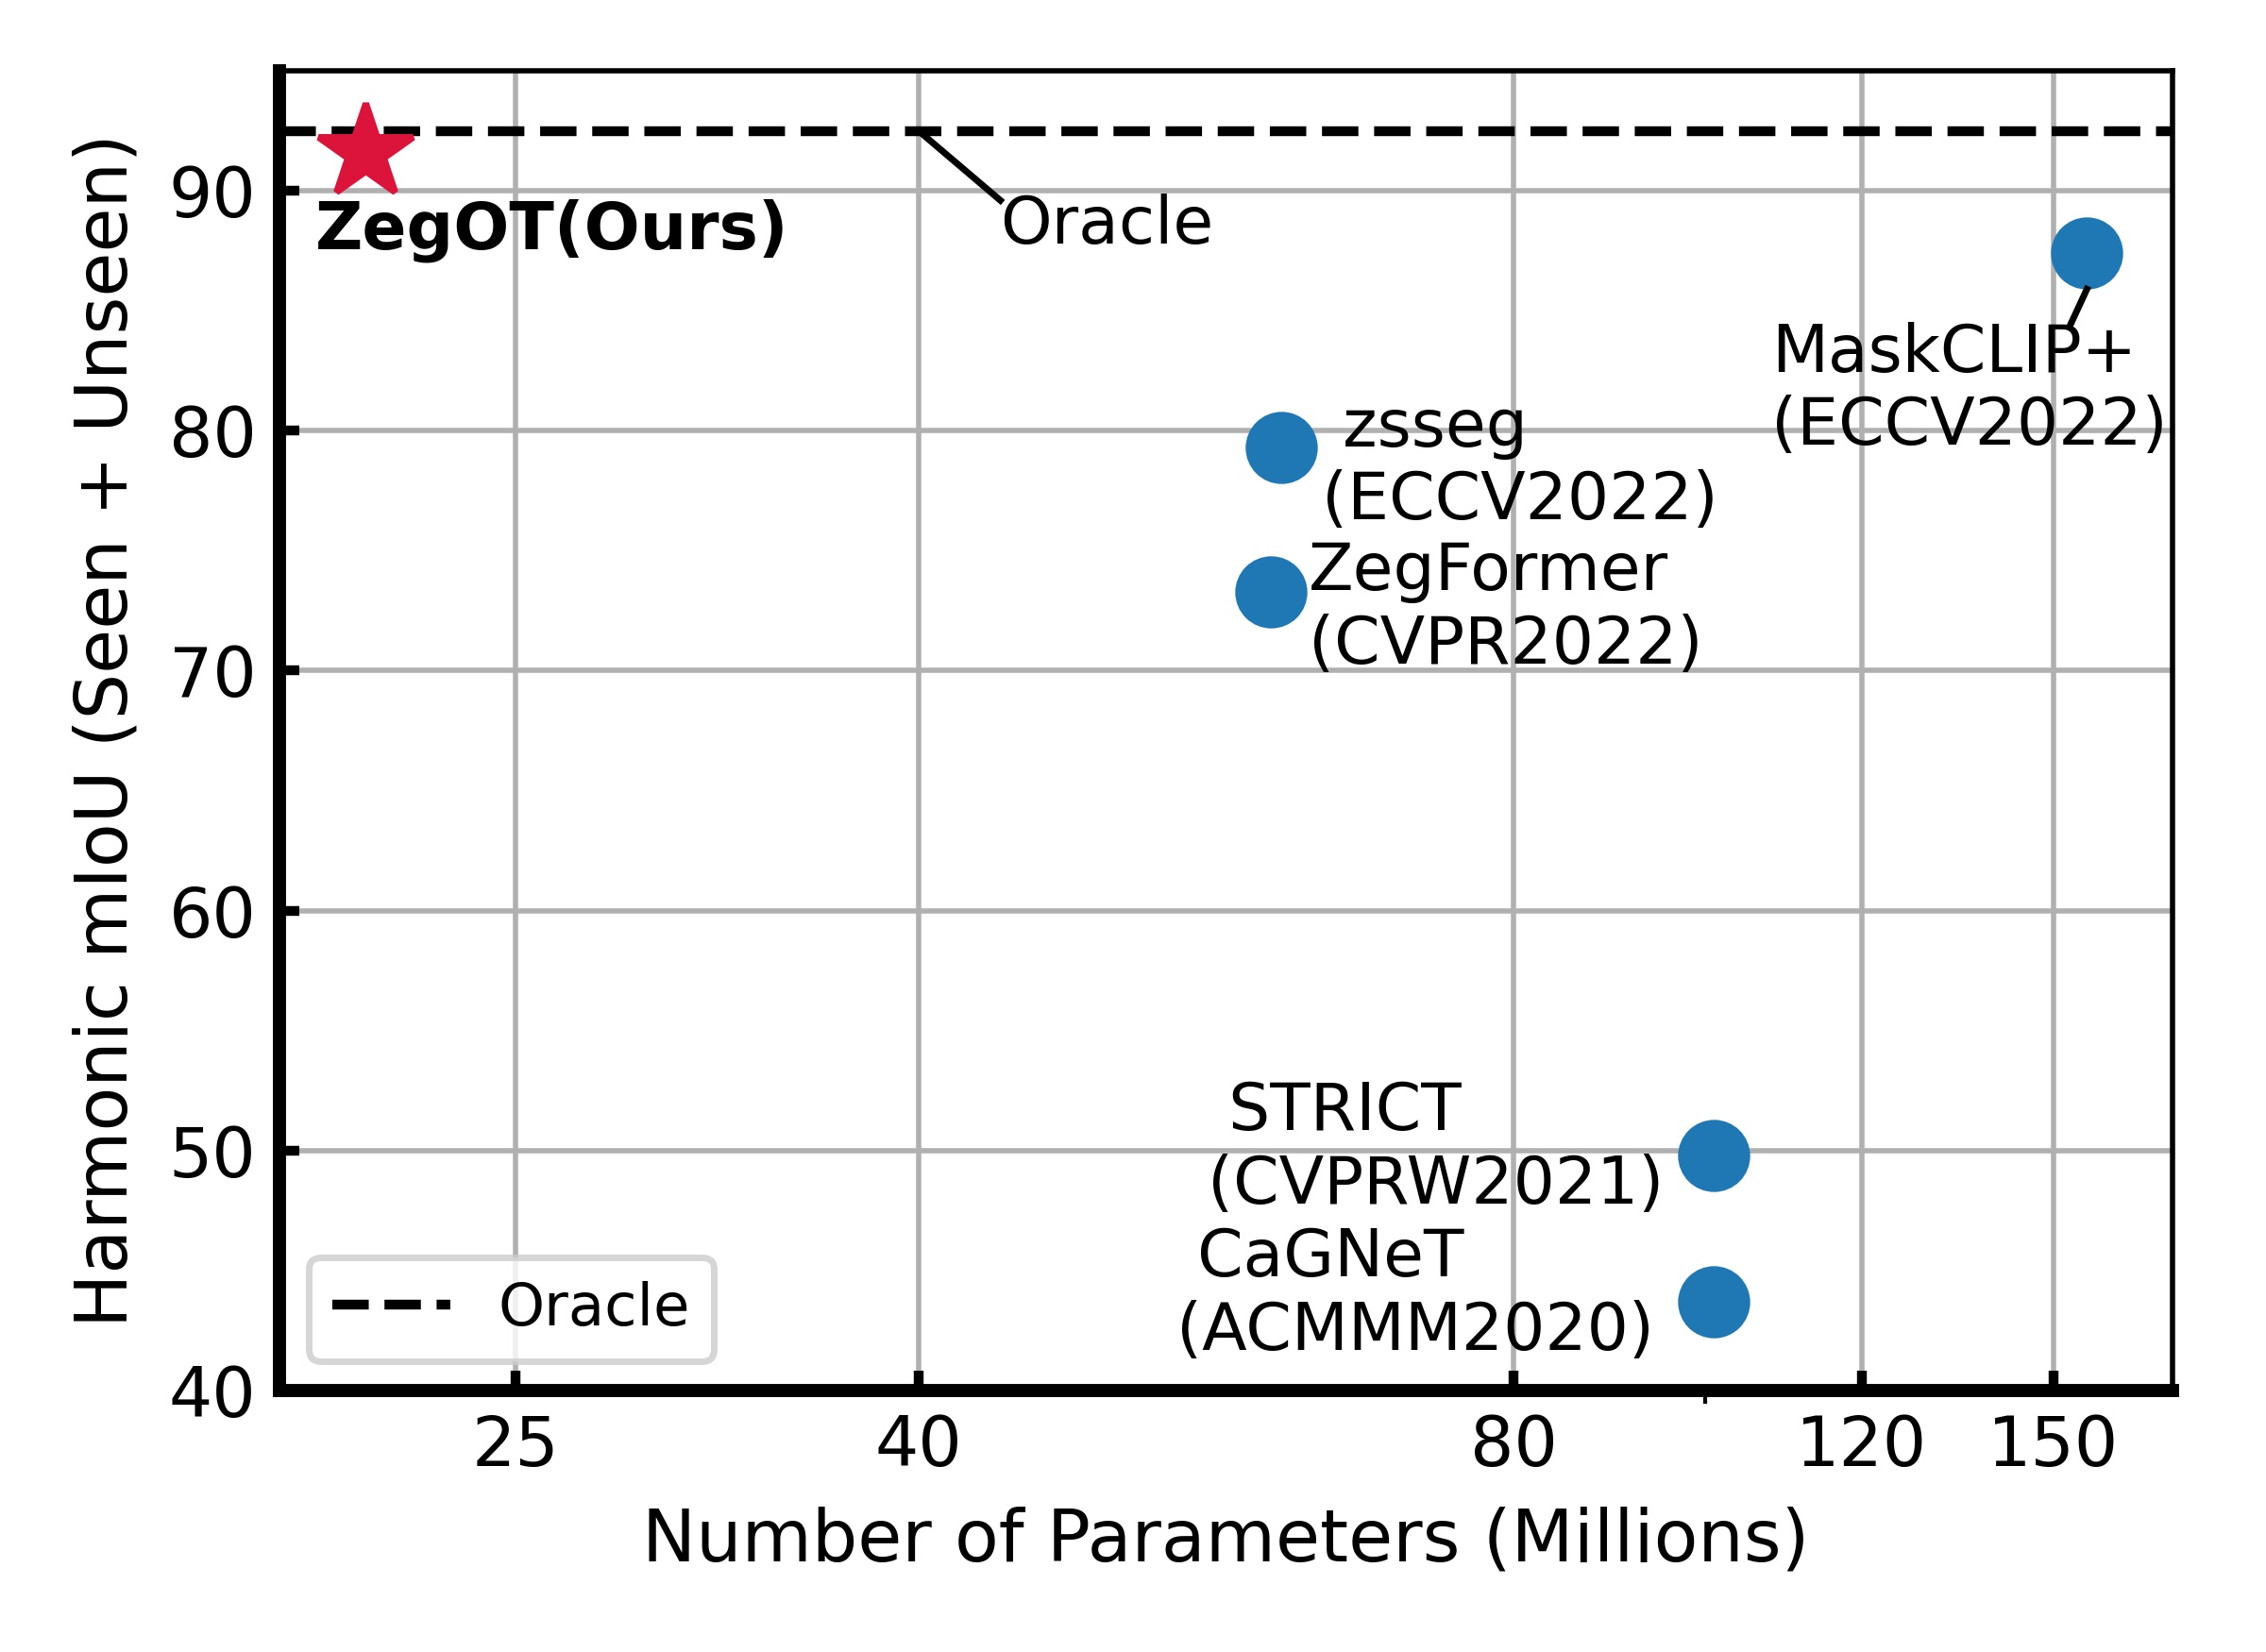
\includegraphics[width=0.98\linewidth]{fig/figure1.jpg}
\vspace*{-0.5cm}
%\caption{Performance of CLIP-based semantic segmentation models and their network parameters.}
{\caption{Harmonic mean IoU of various zero-shot semantic segmentation methods over the number of learnable parameters on PASCAL VOC dataset.
Black dashed line indicates the fully supervised learning result of ours. }}
\label{figure1}
\end{center}
\vskip -0.1in
\end{figure}
%%%%%%%%%%%%%%%%%%%%%%%%%%%%%%%%%%%%%%%%%%%%%%%%%%%%%%%%%%%%%%%%%%%%%%%%%%%%%%%



%Existing ZS3 approaches with pre-trained vision-language model can be categorized into two groups: Frozen image encoder with proposal generator-based approaches (FE) and Re-training or Fine-tuning image encoder-based approaches (TE). 
%Suppose that our goal is to learn functional map that transfers from pre-trained image-level prediction domain knowledge $\mathcal{X}$ to the novel pixel-level prediction domain $\mathcal{Y}$, each with the corresponding probability distribution $p(x)$ and $p(y)$. 
%FE approaches approximate $p(x|y) = p_{\theta}(x|y^I)$ by exploiting the $\mathcal{Y}$ domain knowledge with proposal generator from image information $y^I$. These approaches utilized the capability of image classification with frozen image encoder, $p(x)$. 
%A major drawback of these approaches is that they require training additional image encoder $p_{\theta}(x|y^I)$ to generate region proposals, resulting in high-cost memory complexity. Also, these approaches are highly dependent on the frozen image encoder, which are not specialized for dense prediction.


Suppose that our goal is to learn a functional map that transfers the pre-trained image-level domain $\mathcal{X}$ knowledge to the novel pixel-level domain $\mathcal{Y}$. %To adapt the pre-trained model into a downstream task of novel domain $\mathcal{Y}$, it requires learning additional models or leveraging a novel domain knowledge as illustrated in Table~\ref{table:intro}. 
To achieve this goal, various approaches have been explored by training additional models or leveraging a novel domain knowledge, 
as indicated in Table~\ref{table:intro}.
%For example, it is essential to train image decoder for dense prediction tasks in all of the approaches.
In general, existing ZS3 approaches based on pre-trained VLM can be categorized into two groups: Frozen image encoder with learnable proposal generator-based approaches (FE) \cite{ding2022zegformer, xu2021zsseg}, and trainable image encoder-based approaches (TE) covering re-training or fine-tuning \cite{rao2022denseclip, zhou2022zegclip}. 


%%%%%%%%%%%%%%%%%%%%%%%%%%%%%%%%%%%%%%%%%%%%%%%%%%%%%%%%%%%%%%%%%%%%%%%%%%%%%%%


FE approaches exploit the $\mathcal{Y}$ domain knowledge through image information from the proposal generator. These approaches utilize the capability of image-level classification in the frozen image encoder.
A major drawback of FE approaches is that they require an additional trainable image encoder to generate region proposals, which leads to high-cost memory complexity. Also, FE performance is highly dependent on the frozen VLM, which is not tailored for pixel-level dense prediction.
%TE approaches explicitly address this limitation by learning the image encoder $p_{\phi}(x)$ for dense prediction, $\textit{i.e}$ via estimating $p(y|x) = p(x|y^{T})\frac{p_{\phi}(x)}{p_{\Theta}(y)}$ by replacing $p(x)$ with $p_{\phi}(x)$ and exploiting $\mathcal{Y}$ domain knowledge through text or class information $y^{T}$. 
On the other hand, TE approaches explicitly address the VLM dependency issue by directly training another image encoder for dense prediction and exploiting $\mathcal{Y}$ domain knowledge through class-driven text information.
Compared to FE approaches, leveraging novel domain knowledge through textual information is simple and efficient in terms of complexity.  
%Since these approaches are learned for a specific domain, they showed superior performance for corresponding tasks.
Since TE approaches are learned for a specific domain, they achieve superior performance compared to FE approaches for the corresponding ZS3 task.
%However, they also suffer from high-cost issues due to that inevitable structure that needs to learn $p_{\phi}(x)$. 
However, TE approaches also suffer from high computational cost due to the learnable image encoder. %, which is inevitable.}

%%%%%%%%%%%%%%%%%%%%%%%%%%%%%%%%%%%%%%%%%%%%%%%%%%%%%%%%%%%%%%%%%%%%%%%%%%%%%%%
%% Front Comparison Table

\begin{table}[!t]
\caption{Systemic analysis of ZegOT compared to baseline CLIP-based semantic segmentation models.}
\label{table:intro}
\vskip 0.1in
\begin{center}
\resizebox{0.98\linewidth}{!}{
\begin{tabular}{lccccr}
\toprule
\multirow{2}{*}{Model}  & Proposal & CLIP module & Additional & Multiple &  \multirow{2}{*}{\#Params} \\
& generator & retrain/fine-tune & backbone & text prompt & \\
\cmidrule(r){1-1} \cmidrule(lr){2-5} \cmidrule(l){6-6}
ZegFormer~\cite{ding2022zegformer} &  \checkmark  & \xmark & \xmark & \xmark & 41M \\
zsseg~\cite{xu2021zsseg}     &  \checkmark  & \xmark &  \xmark & \xmark  & 61M  \\
DenseCLIP~\cite{rao2022denseclip} & \xmark &  \checkmark  & \xmark & \xmark & 105M \\
ZegCLIP~\cite{zhou2022zegclip}   & \xmark &  \checkmark  & \xmark & \xmark & ~130M \\
MaskCLIP+~\cite{zhou2022maskclip} & \xmark & \xmark & \checkmark & \xmark & 140M \\
\cmidrule(r){1-1} \cmidrule(lr){2-5} \cmidrule(l){6-6}
\textbf{ZegOT (ours)} &  \xmark  &  \xmark &  \xmark &  \checkmark & \textbf{21M} \\
\bottomrule
\end{tabular}
}
\end{center}
\vskip -0.1in
\end{table}

%The most natural solution is that train only the image decoder and text prompt 
One of the most naive solutions  could be to let the image decoder and text prompt as only learnable parts, while keeping
the VLM image encoder and text encoder frozen.
However, this solution is problematic because the text prompt and image embedding are not effectively aligned since it only utilizes global alignment between image-text. %by using only the global feature. 
%In this paper, as shown in Table~\ref{table:intro}, we propose a cost-effective framework with multiple text prompts, which fully exploits the deeply aligned vision and language embeddings in all the layers without further re-training or tuning. 

To address this,  here we present a cost-effective framework with learnable multiple text prompts which fully exploits both the global and local alignment between vision and language features from deep layers of the frozen VLM without further re-training or tuning (see Table~\ref{table:intro}). 
% 이거 예시야? 아님 설명인가? >> i.e., ?
%\textit{i.e.,} via mapping $p(y|x) = p(x|y^T_{N})\frac{p_{\Theta}(y)}{p^{\ast}(x)}$, where  $y^T_{N}$ denotes class-driven text knowledge with multiple prompts $N$ and $p^{\ast}(x)$ is the image encoder after dense alignment.
%In the setting with frozen image encoder and text encoder, 
%One of the technical difficulties toward this goal is that 
However, in the frozen VLM setting,  % Intro는 현재 시제로 다 통일할게용
%we observe that the multiple text prompts are often overfitted on seen classes, leading to inferior performance on unseen classes. Surprisingly, we find that incorporating optimal transport theory into our framework can be a promising solution by bridging the knowledge of learned classes to novel classes. 
simply introducing the multiple text prompts is problematic, since the learned text prompts can be converged to represent similar semantic features. %leads that all prompts tend to learn for representing the same semantic feature. 
Surprisingly, we found that optimal transport (OT) theory  can provide a solution, by allowing each prompt to efficiently focus on different semantic features, producing optimally aligned pixel-text score maps. %by aligning pixel-text score maps and by allowing each prompt to view different semantic features. 
The aligned score map by OT can tolerate domain shift between different class distributions, leading to robust segmentation performance on unseen classes. %to robustness for the performance of unseen classes.
More specifically, we initially optimize the optimal transport plan between multiple text prompts and the frozen image embeddings on seen classes, and then utilize the optimized transport plan to predict pixel-text score maps for both seen and unseen classes. This allows us to achieve the state-of-the-art (SOTA) performance on both seen and unseen classes, as shown in Figure~\ref{figure1}.    


Our contributions can be summarized as:
\begin{itemize}
\item We propose a cost-effective ZegOT that learns multiple text-prompts while keeping the entire VLM frozen, which allows our model to fully leverage highly aligned vision and language information for zero-shot semantic segmentation tasks.
\item %Despite the effectiveness, %
In ZegOT,
the proposed multi prompt optimal transport solver module
 closely matches the distribution between image embeddings from the frozen VLM and the learnable text-prompts despite its cost-effectiveness.
 %Extensive experiments on three challenging datasets prove that our ZegOT achieves the state-of-the-art performance for zero-shot semantic segmentation tasks, confirming the  distribution transport of our model.
\item {Through extensive experiments on three benchmark datasets, we demonstrate that our ZegOT achieves SOTA performance for zero-shot semantic segmentation tasks while requiring only $\times$7 fewer parameters compared to the previous SOTA approach.}
\end{itemize}







%%%%%%%%%%%%%%%%%%%%%%%%%%%%%%%%%%%%%%%%%%%%%%%%%%%%%%%%%%%%%%%%%%%%%%%%%%%%%%%
%%%%%%%%%%%%%%%%%%%%%%%%%%%%%%%%%%%%%%%%%%%%%%%%%%%%%%%%%%%%%%%%%%%%%%%%%%%%%%%
\section{Related Work}
%Please use no more than three levels of headings.

\subsection{Zero-shot Semantic Segmentation}

Semantic segmentation for large-scale vocabulary needs a labor-intensive pixel-level annotation process, which leads a label-imbalance issue, \textit{i.e.,} not all the categories from the large vocabulary are annotated in the training dataset.
Zero-shot semantic segmentation (ZS3) solves this label-imbalance problem by generalizing labeled (seen) class knowledge to predict new (unseen) class information \cite{bucher2019zero}. 
Recent success of CLIP \cite{radford2021clip} accelerates advancement of ZS3 performance by utilizing aligned knowledge between the image encoder and the class-driven text encoder. Zhou et al. \cite{zhou2022zegclip} successfully bridges the performance gap between the seen and unseen classes by utilizing CLIP model as a backbone feature extractor for dense-level image-text alignment.

ZS3 can be performed by either inductive or transductive settings. Compared to traditional inductive zero-shot setting where class names and pixel-level annotations of unseen classes are both unavailable during training \cite{ding2022zegformer}, a newly introduced transductive setting boosts the ZS3 performance by utilizing unseen class names and self-generated pseudo labels guided by the model itself during training \cite{gu2020cagnet, xu2021zsseg, pastore2021strict, zhou2022zegclip, zhou2022maskclip}. Accordingly, our ZegOT basically follows the transductive ZS3 setting.


%%%%%%%%%%%%%%%%%%%%%%%%%%%%%%%%%%%%%%%%%%%%%%%%%%%%%%%%%%%%%%%%%%%%%%%%%%%%%%%
%% Proposed Schematic

\begin{figure*}[ht]
\vskip 0.1in
\begin{center}
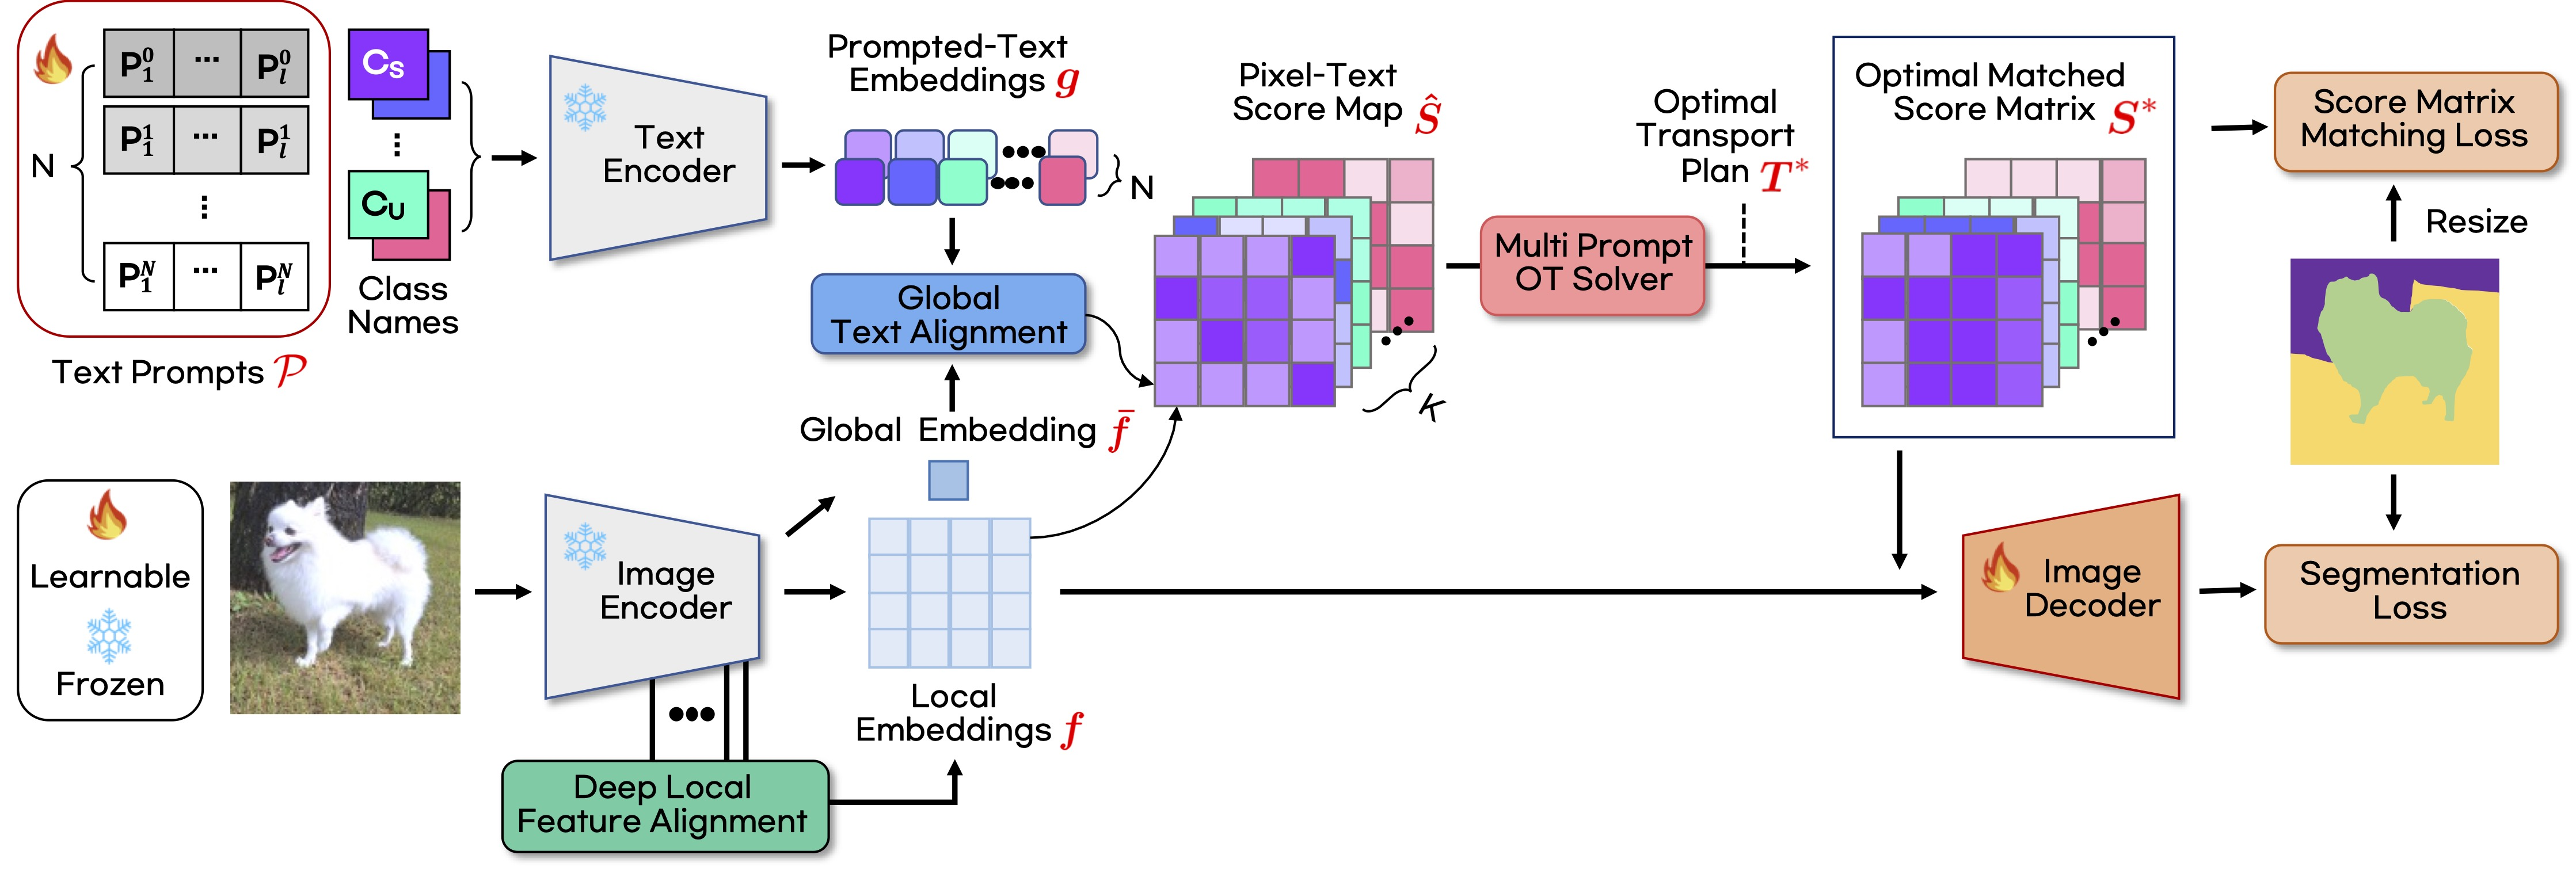
\includegraphics[width=0.97\linewidth]{fig/main.jpg}
\caption{Overall pipeline of our proposed ZegOT for zero-shot semantic segmentation. The only learnable parts are the multiple text prompts $\mathcal{P}$ and the image decoder, while entire CLIP encoder modules are frozen.}
\label{fig_main0}
\end{center}
\vskip -0.1in
\end{figure*}

%%%%%%%%%%%%%%%%%%%%%%%%%%%%%%%%%%%%%%%%%%%%%%%%%%%%%%%%%%%%%%%%%%%%%%%%%%%%%%%


\subsection{Prompt Learning}
Prompt learning was initially introduced in the field of Natural Language Processing (NLP), which efficiently adapts large-scale model knowledge to various downstream tasks.
Rather than using traditional self-supervised learning paradigm,  \textit{i.e.,}  pre-train and fine-tune the large-scale model to transfer the knowledge to downstream tasks, 
%Rather than the conventional
%which first pre-trains a large-scale model and then fine-tunes the head with task-specific objective functions, 
the prompt learning formulates the downstream adjustment problem by training light-weight optimal textual prompts~\cite{petroni2019language,shin2020autoprompt,jiang2020can,liu2021gpt}. %problem of adjusting downstream tasks
Compared to the fine-tuning method, text prompts-driven downstream adaptation is efficient, but still alleviates the domain shift problem that occurs between the pre-trained domain and the downstream domain. 
Recently, introducing a set of learnable text prompts into the frozen VLM achieved superior performance in various computer vision (CV) tasks~\cite{zhou2022learning, zhou2022conditional, gao2021clip,rao2022denseclip}. 
Visual Prompt Tuning (VPT) is also a novel solution that introduces trainable image prompts to each layer of a transformer encoder~\cite{jia2022visual}, %parameter in each layer of transformers
which can be transferred to various downstream tasks~\cite{zang2022unified,sohn2022visual,liu2022prompt}. 
However, VPT requires high memory consumption, which is comparable to the re-training method. Our method uses only text prompts to adapt to the ZS3 task, which leads to a memory-efficient advantage.

\subsection{Optimal Transport}
Optimal transport (OT) is a general mathematical framework to evaluate correspondences between two distributions. 
% then enable us to a, to neural networks 
%Owing 
Thanks to the luminous property of distribution matching, the optimal transport  has received great attention in various computer vision tasks, such as domain adaptation~\cite{flamary2016optimal}, semantic correspondence problem~\cite{liu2020semantic}, graph matching~\cite{xu2019scalable,xu2019gromov}, and cross-domain alignment~\cite{chen2020graph}, etc.  
%The work most related to ours is 
Among various methods, Sinkhorn algorithm can efficiently solve the OT problem through entropy-regularization~\cite{cuturi2013sinkhorn}, and it can be directly applied to deep learning frameworks thanks to the extension of Envelop Theorem~\cite{peyre2019computational}. 
Prompt Learning with Optimal Transport (PLOT) \cite{chen2022prompt} is mostly related to ours, which optimizes the optimal transport distance to align visual features and text features by the Sinkhorn algorithm given trainable multiple text prompts. However, PLOT only considers a few-shot image classification problem, while we apply the optimal transport theory to a zero-shot dense prediction problem to focus on
specific attributes of semantic objects, which facilitates ZS3.  %and thus 

% %%%%%%%%%%%%%%%%%%%%%%%%%%%%%%%%%%%%%%%%%%%%%%%%%%%%%%%%%%%%%%%%%%%%%%%%%%%%%%%
% %%%%%%%%%%%%%%%%%%%%%%%%%%%%%%%%%%%%%%%%%%%%%%%%%%%%%%%%%%%%%%%%%%%%%%%%%%%%%%%
\section{Methods}
\label{methods}
As illustrated in Figure~\ref{fig_main0}, our proposed ZegOT is composed of frozen text/image encoder modules with trainable text prompts, a global text alignment (GTA) module, an image decoder module and a multi prompt optimal transport solver (MPOT) module. A primary goal of ZegOT is to segment objects belongs to both seen classes $\mc{C}_S$ and unseen classes $\mc{C}_U$, \textit{i.e.,} $\mc{C} = \mc{C}_{S} \cup \mc{C}_U$, under the transductive ZS3 setting. % \in \mathbb{R}^K
Note that $\mc{C}_S \cap \mc{C}_U = \emptyset$ and 
both annotations and class names of $\mc{C}_S$ are available, but the only class names of
$\mc{C}_U$ are known during training. 
We introduce two novel methods into ZegOT to learn dense vision-language alignment in a cost-effective way: 1) prompt-guided deep text-pixel alignment and 2) multi prompt optimal transport solver.


\subsection{Prompt-guided Deep Text-Pixel Alignment}

 \paragraph{Multiple Text Prompt Learning}

%  Let $C$ as the dimension of the embedding and $l$ as the length of context token.
%  Given a word embedding of the class name $\bs{c}_k \in \mathbb{R}^{1 \times C}$ and learnable context vectors $\mbf{P} = [P_1,P_2,\dots,P_l] \in \mathbb{R}^{l \times C}$,
%  the single textual prompt can be described as $\bs{t}_{k} = \{\mbf{P}, \bs{c}_{k}\} \in \mathbb{R}^{(l+1) \times C}, \, k=1, \dots, K$, where the context vectors $\mbf{P}$ are shared throughout all the classes.
% To fully leverage the CLIP pre-trained knowledge, we can initialize multiple textual prompts $\bs{t}_{k} =\{\mbf{P}^n, \bs{c}_{k}\}^N_{n=1} \in \mathbb{R}^{(l+1) \times C \times N}, \, k = 1,\dots K$, where $N$ denotes the number of text prompts. 
 To fully leverage the CLIP pre-trained knowledge, we make $N$ text prompts $\mathcal{P} = \{\bs{P}^{i}|^N_{i=1}\}$ as only trainable context tokens from the text encoder module. \textit{i.e.,} $\bs{P}^i =[P^i_1,P^i_2, \cdots, P^i_l],$ where $l$ denotes the length of the context tokens. 
 The randomly initialized multiple text prompts $\mathcal{P}$ are identically prepended to $K$ tokenized class names as $\mathcal{T} = \{\{\mathcal{P}, \bs{c}^k\}|^K_{k=1}\}$, where $\{\bs{c}^k|_{k=1}^K\} \subset \mc{C}$ is the word embedding of each class name. Note that the text prompts $\mathcal{P}$ are shared throughout all the class names. The $N$-prompted class names $\mathcal{T}$ are then encoded into text embeddings $\bs{g} = E_{\text{text}}(\mathcal{T}) \in {\mathbb{R}^{KN \times D}}$, where $E_{\text{text}}$ is the frozen text encoder, $D$ denotes the embedding dimension. On the other hand, an input image is encoded through the frozen CLIP image encoder layer to yield global image embedding $\bs{\bar{f}}_L \in \mathbb{R}^{1 \times D}$ and local image embeddings {$\bs{f}_L \in \mathbb{R}^{H_LW_L \times D}$, where $H_{L}$ and $W_{L}$ are the height and width of the local image embeddings from $L$-th layer.


In this work, we define variants of desirable pixel-text aligned score matrices as: 
%Then, a desirable pixel-text aligned score matrix $\bs{S}$ can be computed using $\bs{g}$ and $\bs{f_L}$ as: 
\begin{align}
	%\bs{S} = \bs{{\bs{f_L}\bar{g}}}^{\top}, \quad 
	\bs{S}_i = \bs{f}_i \bs{g}^{\top},%\quad \bs{\hat S} = \bs{f_L} {\bs{g}^{\top}_{GA}},\quad 
	\bs{\hat S}_i = \bs{f}_i {\bs{g}^{\top}_{GA}},\quad i=1,\cdots, L
	\label{eq:score}
\end{align} 
$$\bs{S}^{\ast}_i= \bs{T}^{\ast}_i \odot\bs{\hat S}_i,$$
where 
$$ \bs{g}_{GA} = \mathcal{Q} (cat\left[\bs{\bar{f_L}}  \odot \bs{{g}}, \bs{{g}} \right] )$$
where $\bs{S}_i, \bs{\hat S}_i \in \mathbb{R}^{H_LW_L \times KN}$ is the $i$-th score matrices using $\bs{g}$, and  $\bs{g}_{GA}$, respectively. $\bs{g}_{GA} \in \mathbb{R}^{KN \times D}$ is the text embeddings by global text aligment and will be explained in later, 
$\bs{f}_i \in \mathbb{R}^{H_LW_L \times D}$ is the $i$-th intermediate local image embeddings from the $i$-th hidden image encoder layer. Here, %$\bs{g}^{\top}$ and $\bs{g}_{GA}^{\top}$  refers to the transpose operation that views $\mathbb{R}^{(K \times N) \times D}$ as $\mathbb{R}^{KN \times D}$,
Here, the superscript $^{\top}$ refers to the transpose operation,
$\bs{S}^{\ast}_i \in \mathbb{R}^{H_LW_L \times KN}$ is the refined score matrix by optimal transport map $\bs{T}^{\ast}_i$ and will be discussed in Sec~\ref{MPOT}. $\mathcal{Q}$ denotes a linear layer for matching the concatenated embedding dimension to the original dimension, and $\odot$ is the Hadamard product. $\bs{f}_L$ and $\bs{g}$ are $\mathcal{L}_2$ normalized along the embedding dimension. 

The score matrices in $\eqref{eq:score}$ can be either directly matched to the pixel-level annotation labels, or %inptted
fed into the image decoder as an intermediate feature to predict segmentation maps as:
\begin{align}
\mbf{Y} = D_{\theta}(cat[\{\mathcal{M}(\bs{S}_i)|_{i=1}^{L}\},\mathcal{M}(\bs{S}_L)]),  \label{eq:predict1} \\ 
\mbf{\hat Y} =  D_{\theta}(cat[\{\mathcal{M}(\bs{\hat S}_i)|_{i=1}^{L}\}, \mathcal{M}(\bs{\hat S}_L)]),  \label{eq:predict2}\\
\asty = D_{\theta}(cat[\{\mathcal{M}(\bs{\hat S}_i)|_{i=1}^{L}\},  \mathcal{M}(\bs{S}^{*}_L)]).
 \label{eq:predict3}
\end{align}
%\begin{eqnarray}
%\bs{S^{\ast}} = \;<\bs{T^{\ast}_L},\bs{\hat S_L}>, \; 
%\hat Y^* =  D_{\theta}(cat[\{\mathcal{M}(\bs{\hat S}_i)|_{i=1}^{L}\},  \mathcal{M}(\bs{S^\ast}_L)])% \bs{S^{\ast}}])
%\label{shallow}
%\end{eqnarray}
%$$\bs{S^{\ast}}= \bs{T^{\ast}_L} \odot\bs{\hat S_L}$$
where $\mbf{Y, \hat Y}, \asty \in \mathbb{R}^{HW \times K}$ is outputs of the decoder using $\bs{S}_i$, $\bs{\hat S}_i$, and $\bs{S}^{\ast}_L$, and 
$\mathcal{M}$: $\mathbb{R}^{H_LW_L \times KN} \rightarrow \mathbb{R}^{H_L W_L \times K}$ is operation which first reshape $\mathbb{R}^{H_L W_L \times KN} \rightarrow \mathbb{R}^{H_L W_L \times K \times N}$ and summation the marix along the $N$ dimension. \textit{e.g.,} $\mathcal{M}(\bs{\hat S}_i) \in \mathbb{R}^{H_L W_L\times K}$, $D_{\theta}$ is the trainable image decoder, and \textit{cat} is the concatenation operator, and $H$ and $W$ are the height and width of image, respectively. 
$\mbf{Y}$ is  prediction without any our proposed component, and $\mbf{\hat Y}$ is the prediction of our baseline model, and $\asty$ is the prediction of ZegOT.
The details of $\asty$ will be discussed in Sec.~\ref{MPOT}. 
The used notation is summarized in Table~\ref{tab:notation}(Appendix~\ref{apppendix:notation}).}
    
 \paragraph{Global Text Alignment (GTA)}
 The local image embeddings $\bs{f}_L$ inherently contain the text-image aligned knowledge of CLIP. 
However, when pre-training, the global image embedding $\bs{\bar{f}}_L$  and the text embeddings  $\bs{g}$ comprise the cosine similarity score which is maximized through contrastive learning so that $\bs{\bar{f}}_L$ contains richer pixel-text aligned information than $\bs{f}_L$. 
Thus, we further exploit $\bs{\bar{f}}_L$ in the GTA module to compute the score matrices $\{\bs{\hat S}_i\}_{i=1}^{L}$  by employing an idea of relation descriptor method \cite{zhou2022zegclip} in \eqref{eq:score}. 
 %The globally aligned score matrix can be reformulated as:
%Specifically, the score matrix passing through the GTA module can be reformulated as: 
% \begin{align}  
 % \add{		\bs{\hat S} = \bs{f_L} {\bs{g}^{\top}_{GA}}, \quad \bs{g}_{GA} = \mathcal{Q} (cat\left[\bs{\bar{f_L}}  \odot \bs{\bar{g}}, \bs{\bar{g}} \right] )
 %		\label{eq:score_ga}}
 %\end{align} 
 %where  $\bs{\hat S} \in \mathbb{R}^{H_{L}W_{L} \times KN}$ is the score matrix using GTA, {$\bs{g}_{GA} \in \mathbb{R}^{KN \times D}$} is the globally aligned text embedding and $\mathcal{Q}$ denotes a linear layer for matching the concatenated embedding dimension to the original dimension, and $\odot$ is the Hadamard product.

\paragraph{Deep Local Feature Alignment (DLFA)}
 Meanwhile, Feature Pyramid Network (FPN) \cite{lin2017fpn} is a common choice for segmentation decoder, 
where high-level semantic features from deep encoder layers comprise a latent feature for the following image decoder.
 Our ZegOT also adopts FPN,  but we fully align the extracted intermediate local embeddings from the frozen image encoder with the globally aligned text embedding $\bs{g}_{GA}
 $. Accordingly, the model prediction with DLFA can be described as $\mbf{\hat Y}$ in ~\eqref{eq:predict2}.
%\begin{eqnarray}
%\add{\hat y =  D_{\theta}(cat[\{\mathcal{M}(\bs{\hat S}_i)|_{i=1}^{L}\}, \mathcal{M}(\bs{\hat S})]),
 %\quad \bs{\hat S}_i = \bs{f}_i {\bs{g}^{\top}_{GA}} }
%\label{eq:final}
%\end{eqnarray}
%where $\bs{\hat S}_i  \in \mathbb{R}^{H_{L}W_{L} \times KN}$ is the $i$-th score matrix that aligns $\bs{f}_i$ and $\bs{g}_{GA}$.
%the $i$-th aligned score map from the $i$-th image encoder layers. 
Through the simple arithmetic calculation, the entire hidden image embeddings extracted from the frozen CLIP encoder can be deeply aligned with both the global image and text embeddings without any further learnable parameters.




\subsection{Multi Prompt Optimal Transport Solver}
\label{MPOT}
%Now, the key idea of ZegOT is to
%learn the mapping $D_\theta$ in Eqs.~\eqref{eq:predict} and \eqref{eq:final} through the optimal transport
%since the OT can effectively align the distributions, producing optimally aligned pixel-text score map.


\paragraph{Optimal Transport Problem}
Optimal transport aims to minimize the transport distance %optimize a minimum transport distance 
between two probability distributions. In this paper, we only consider discrete distribution which is closely related to our framework. We assume that discrete empirical distributions $\bs{\mu}$ and $\bs{\nu}$ are defined on probability space $\mathcal{F}, \mathcal{G} \in \Omega$, respectively, as follows:
\begin{align}
\bs{\mu} = \sum^{M}_{i=1} p_{i} \delta_{f_{i}}, \quad \bs{\nu} = \sum^{N}_{j=1} q_{j} \delta_{ g_{i}}, 
\end{align}
where $\delta_f$ and $\delta_g$ denote Dirac functions centered on $\bs{f}$ and $\bs{g}$, respectively, $M$ and $N$ denote the dimension of the empirical distribution. %embedding space. 
The weight vectors $\boldsymbol{p} = \{p_i\}^M_{i=1}$ and $\boldsymbol{q} = \{q_i\}^{N}_{j=1}$  belong to the $M$ and $N$-dimensional simplex, respectively, \textit{i.e.}, $\sum^{M}_{i=1} p_i = 1$, $\sum^{N}_{j=1} q_j = 1$. The discrete optimal transport problem  can be then formulated as: 
\begin{eqnarray}
\bs{T}^{\ast} = \underset{\bs{T}\in \mathbb{R}^{MXN}}{\arg{\min}} \sum^{M}_{i=1}\sum^{N}_{j=1}\bs{T}_{ij} \bs{C}_{ij} \nonumber \\ \textrm{s.t.} \quad \bs{T}\bs{1}^{N} = \bs{\mu}, \quad \bs{T}^{\top}\bs{1}^{M} = \bs{\nu} .
\label{DOT}
\end{eqnarray}
Here,
$\bs{T}^{\ast}$ is called the optimal transport plan, which is learned to minimize %optimize 
the total distance between the two probability vectors. $\bs{C}$ is the cost matrix which represents the distance between $\boldsymbol{f}_i$ and $\boldsymbol{g}_j$, \textit{e.g.,} the cosine distance $\bs{C}_{ij}$ = 1 - $\frac{\bs{f}_i\bs{g}^{\top}_j}{\|\bs{f}_i\|_2 \|\bs{g}_j\|_2}$, and $\bs{1}^{M}$ refers to the $M$-dimensional vector with ones. 

However, solving the problem~\eqref{DOT} costs $O(n^3\log n)$-complexity ($n$ proportional to $M$ and $N$), which is time-consuming. 
This issue can be efficiently solved by entropy-regularizing the objective, called the Sinkhorn-Knopp (or simply Sinkhorn) algorithm~\cite{cuturi2013sinkhorn}. In
Sinkhorn algorithm, the optimization problem is reformulated as:
\begin{eqnarray}
\bs{T}^{\ast} = \underset{\bs{T}\in \mathbb{R}^{MXN}}{\arg{\min}} \sum^{M}_{i=1}\sum^{N}_{j=1}\bs{T}_{ij}\bs{C}_{ij} - \lambda H(\bs{T}) \nonumber \\ \textrm{s.t.} \quad \bs{T}\bs{1}^{N} = \bs{\mu}, \quad \bs{T}^{\top}\bs{1}^{M} = \bs{\nu} .
\label{Sinkhorn}
\end{eqnarray}
where $H(\bs{T})$ = $\sum_{ij} \bs{T}_{ij} \log \bs{T}_{ij}$ and $\lambda > 0$ is the regularization parameter.
The problem \eqref{Sinkhorn} is a strictly convex optimization problem, and thus we have an optimization solution with fewer iterations as follows: %a few iterations.
\begin{eqnarray}
\bs{T}^{\ast} = \text{diag}(\bs{a}^{t})\exp(-\bold{C}/\lambda)\text{diag}(\bs{b}^{t})
\label{Sinkhorn2}
\end{eqnarray}
where $t$ is the iteration and $\bs{a}^t = \bs{\mu}/ \exp(-\bold{C}/\lambda)\bs{b}^{t-1}$ and $\bs{b}^{t} = \bs{\nu}/\exp(-\bold{C}/\lambda)\bs{a}^{t}$, with the initialization on $\bs{b}^{0}=\bs{1}$.


%%%%%%%%%%%%%%%%%%%%%%%%%%%%%%%%%%%%%%%%%%%%%%%%%%%%%%%%%%%%%%%%%%%%%%%%%%%%%%%
%%  OT

\begin{figure}[t]
\vskip 0.1in
\begin{center}
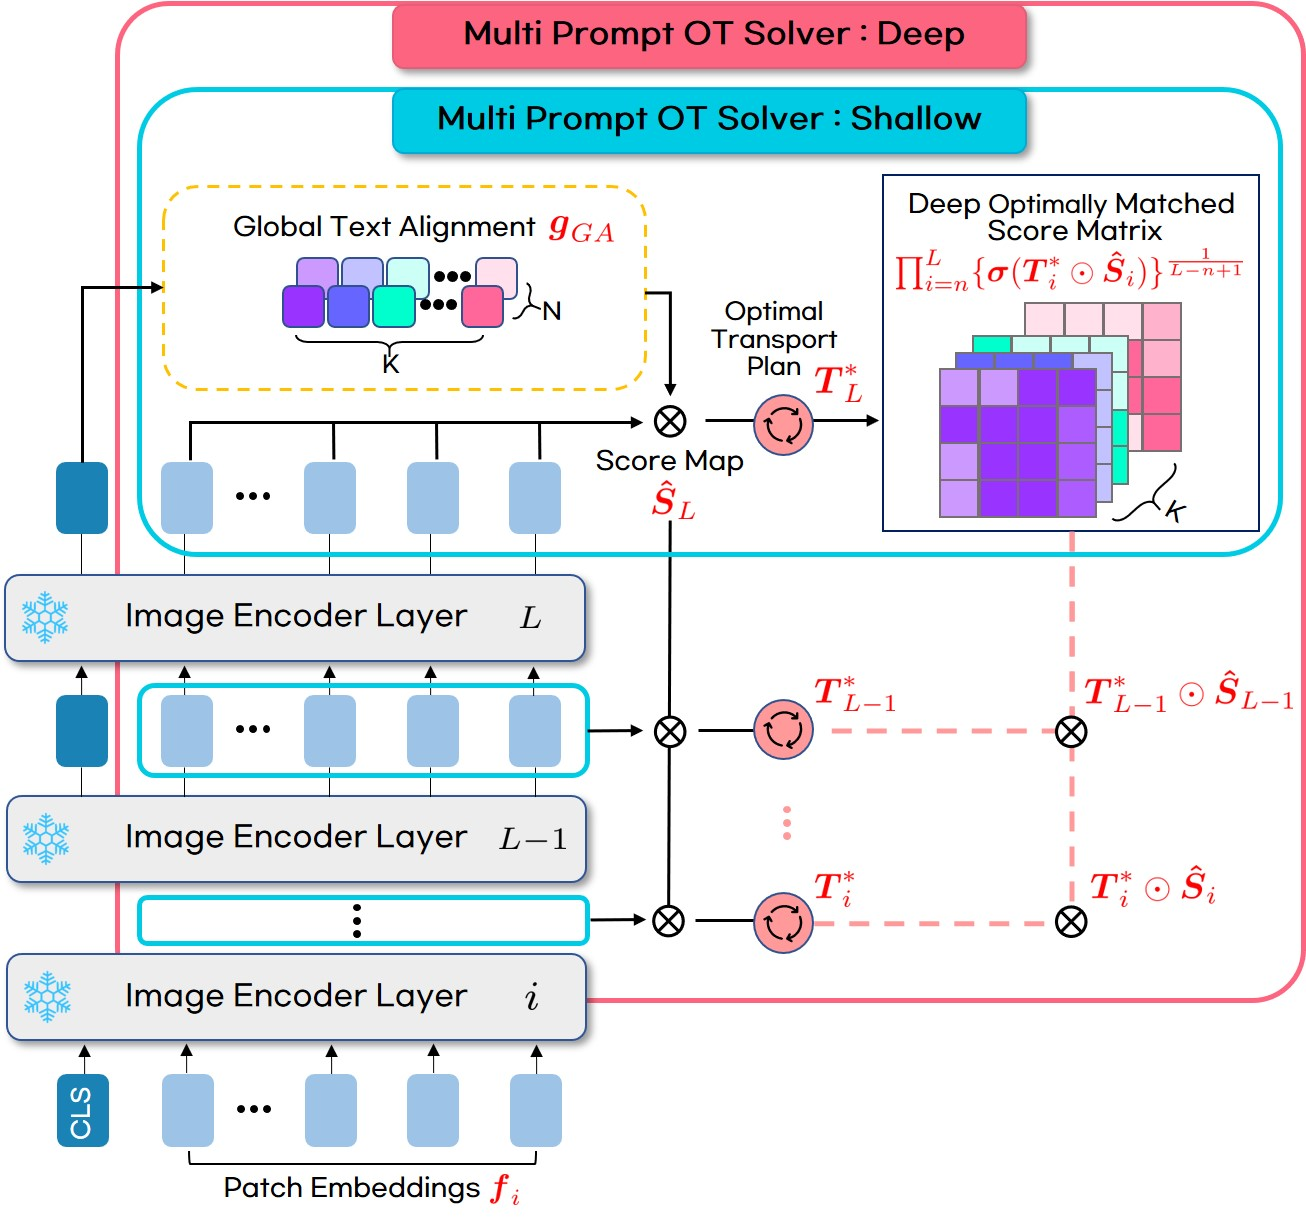
\includegraphics[width=0.95\linewidth]{fig/OT.jpg}
\caption{A schematic diagram of Multi Prompt Optimal Transport (MPOT) solvers including Shallow and Deep variants.}
\label{ot-solver}
\end{center}
\vskip -0.1in
\end{figure}
%%%%%%%%%%%%%%%%%%%%%%%%%%%%%%%%%%%%%%%%%%%%%%%%%%%%%%%%%%%%%%%%%%%%%%%%%%%%%%%


\paragraph{Mulitple Prompt OT Solver (MPOT)}
To incorporate the OT theory into our framework, we define the total cost matrix $\bs{C}$ in ~\eqref{Sinkhorn} using the globally aligned score matrix $\bs{\hat S}_i$ in~\eqref{eq:score}, \textit{i.e.,} 
{$\bs{C}_i  = \bs{1 - \hat S}_i$,} where $\bs{C}_i \in \mathbb{R}^{H_LW_L \times K N}$ denotes the $i$-th cost matrix calculated from $\bs{\hat S}_i$.
Given the cost matrix $\bs{C}_i$, the goal of MPOT is to obtain the corresponding optimal transport plan $\bs{T}^{\ast}_i  \in \{\bs{T}^{\ast}_i\}^L_{i=1}$ as Eq.~\eqref{Sinkhorn2}  {(Here, $M = H_LW_L$, $N= N$ in \eqref{Sinkhorn} and the algorithm in Appendix \ref{algo-ot})}, which is a mapping matrix that maximizes the cosine similarity between the frozen image embedding and the learnable multiple prompts-derived text embeddings.
Depending on the depth of incorporating image encoder layers for the optimization process, we have two ZegOT variants,  $\textit{i.e.,}$ ZegOT-Shallow and ZegOT-Deep, as shown in Figure~\ref{ot-solver}.

\paragraph{ZegOT-Shallow}
%Given the score matrix $\bs{\hat S}_L$ using $L$-th layer, we can calculate the corresponding optimal transport plan {$\bs{T}^{\ast}_L \in \mathbb{R}^{H_{L}W_{L} \times KN }$} as Eq.~\eqref{Sinkhorn2}  {(Here, $M = H_LW_L$, $N= N$ in \eqref{Sinkhorn} and  the algorithm in Appendix \ref{algo-ot})}, which is a mapping matrix that maximizes the cosine similarity between the frozen image embedding and the learnable multiple prompts-derived text embeddings.
As illustrated in Fig~\ref{ot-solver}, ZegOT-Shallow calculate optimal transport plan $\bs{T}^{\ast}_L \in \mathbb{R}^{H_LW_L \times K N}$ in $L$-{th} layer. 
Since our goal is to obtain a pixel-text score matrix that minimizes the total distance between the two image and text embedding spaces, we can reformulate the final score matrix as : %written
\begin{eqnarray}
\bs{S}^{\ast}_L= \bs{T}^{\ast}_L \odot\bs{\hat S}_L
\label{eq:shallow}
\end{eqnarray}
where $\bs{S}^{\ast}_L$ is the refined score matrix wth transport plan $\bs{T}^{\ast}_L$ in $L$-th layer. Then, we can obtain the prediction of ZegOT-Shallow $\asty$ by pluging \eqref{eq:shallow} into \eqref{eq:predict3}.
%\add{where $<\bs{A},\bs{B}> = \mathcal{M}(\bs{A} \odot \bs{B})$ is operator that is similar to the Frobenius inner product along $N$ dimension, $\bs{S}^{\ast}  \in \mathbb{R}^{H_{L}W_{L} \times K}$ is the refined score matrix by the optimal transport map $\bs{T_{L}}^{\ast}$.} %optimal matched

\paragraph{ZegOT-Deep}
Instead of optimizing the transport plan $\bs{T}^{\ast}_L$ just for the single layer as in Eq.~\eqref{eq:shallow},  ZegOT-Deep leverages intermediate image embeddings from the deep image encoder layers  to yield multiple
%Rather than  matching the distribution in only a, ZegOT-Deep leverage MPOT in the multiple intermediate layers and we can obtain several 
transport plans $\{\bs{T}^{\ast}_i\}_{i=n}^L$,
where $\bs{T}_i \in \mathbb{R}^{H_LW_L \times K N}$ and $n$ denotes the starting layer that comprises the multiple transport plans.
%where $n$ denotes the number of initial layer for inserting MPOT. 
%When we combine these optimal transport plans and score maps, 
We apply geometric mean among the multiple transport plans to reflect the knowledge of intermediate score matrices as follows: 
\begin{eqnarray}
\bs{S}^{\ast}_L = \; \prod^{L}_{i=n} \bs{\sigma}\{\bs{S}^{\ast}_i\}^{\frac{1}{d}}, \, \bs{S}^{\ast}_i= \bs{T}^{\ast}_i \odot\bs{\hat S}_i
\label{eq:deep}
\end{eqnarray}
where $d = L - n + 1$ denotes the depth of incorporating image encoder layers, $\bs{\sigma}$ is the sigmoid function if $n\leq i<L$, and the identity function otherwise~(since intensity range of all the score matrix is (-1,1), we conduct Sigmoid for all the intermediate image embeddings except for the last layer).
% (because the intensity range of score maps is (-1,1), we conduct the Sigmoid function into the intermediate layer except for the last layer).
Accordingly, in ZegOT-Deep, the model prediction $\asty$ can be obtained by pluging \eqref{eq:deep} into \eqref{eq:predict3}.
Note that Eq.~\eqref{Sinkhorn2} only contains matrix multiplication and exponential operation, \textit{i.e}, the calculations are fully differentiable, thus the gradients can be back-propagated throughout the entire neural network. 

% %%%%%%%%%%%%%%%%%%%%%%%%%%%%%%%%%%%%%%%%%%%%%%%%%%%%%%%%%%%%%%%%%%%%%%%%%%%%%%%
% %% Sinkhorn Algorithm

% \begin{algorithm}[tb]
%    \caption{Optimal transport matching algorithm by applying Sinkhorn distance}
%    \label{alg:example}
% \begin{algorithmic}
%    \STATE {\bfseries Input:} data $x_i$, size $m$
%    \REPEAT
%    \STATE Initialize $noChange = true$.
%    \FOR{$i=1$ {\bfseries to} $m-1$}
%    \IF{$x_i > x_{i+1}$}
%    \STATE Swap $x_i$ and $x_{i+1}$
%    \STATE $noChange = false$
%    \ENDIF
%    \ENDFOR
%    \UNTIL{$noChange$ is $true$}
% \end{algorithmic}
% \end{algorithm}
% %%%%%%%%%%%%%%%%%%%%%%%%%%%%%%%%%%%%%%%%%%%%%%%%%%%%%%%%%%%%%%%%%%%%%%%%%%%%%%%



\subsection{Training Procedure and Inference}
As dicussed in Section~\ref{methods}, ZegOT follows the transductive ZS3 setting. Similar to the previous SOTA methods~\cite{zhou2022zegclip, zhou2022maskclip}, the entire training schedule is divided into three phases:
Seen classes-guided learning, Pseudo label-guided learning, and Self-training. 
For each phase, ground-truth labels for unseen classes are updated, $\textit{i.e.,}$ ZegOT self-generates labels at once or continuously (see the details of the training phases are described in Appendix \ref{sec_phase}).

\paragraph{Loss Function} \label{sec:loss}
%Model parameters are optimized following two objective function:
%we use the combined three losses
In this work, we combine three different losses which is similar to previous methods as follows:
\begin{align}
&\mathcal{L}_{\text{total}} = \lambda_{\text{CE}} \mathcal{L}_{\text{CE}} + \lambda_{\text{fc}} \mathcal{L}_{\text{fc}} + \lambda_{\text{dc}} \mathcal{L}_{\text{dc}}, 	\\
&\mathcal{L}_{\text{seg}} = \mathcal{L}_{\text{total}}(\asty, \gty), \\
&\mathcal{L}_{\text{score}} = \mathcal{L}_{\text{total}}(\mathcal{M}(\bs{S}^{\ast}_L),\mathcal{R}_{d}(\gty))
\label{losses}
\end{align}
where $\mathcal{L}_{\text{total}}$ denotes the total loss combining different three losses, $\textit{i.e.,}$ $\mathcal{L}_{\text{CE}}$ is the cross entropy loss, $\mathcal{L}_{\text{fc}}$ is the focal loss, and $\mathcal{L}_{\text{dc}}$ is the dice loss, with $\lambda_{\text{CE}}$, $\lambda_{\text{fc}}$, and  $\lambda_{\text{dc}}$ as corresponding hyper-parameters. 
$\mathcal{L}_{\text{seg}}$ is the segmentation loss and $\mathcal{L}_{\text{score}}$ is the score matrix matching loss, where $\asty \in \mathbb{R}^{HW \times K}, \, \mathcal{M}(\bs{S}^*_{L}) \in \mathbb{R}^{H_LW_L\times K}$ are the predictions of our model, and $\mathcal{R}_d:\mathbb{R}^{HW \times K} \rightarrow \mathbb{R}^{H_LW_L \times K}$ is the downsampling operator ($H_LW_L < HW$). $\gty \in \mathbb{R}^{HW \times K}$ is the ground-truth label.
%, where label $\gty$ is phase-adaptively altered for training the unseen classes, as described in Appendix~\ref{sec_phase}.

In the training phase, the following two optimization problems are updated as :
\begin{align}
&\underset{\{\bs{P}^i\}_{i=1}^N} \min \;\mathcal{L}_{\text{prompt}} = \lambda_{\text{seg}} \mathcal{L}_{\text{seg}} + \lambda_{\text{score}} \mathcal{L}_{\text{score}}, \\ &\underset{D_{\theta}} \min \; \mathcal{L}_{\text{Decoder}} = \lambda_{\text{seg}} \mathcal{L}_{\text{seg}}
\label{seg,score_loss}
\end{align}
where $\mathcal{L}_{\text{prompt}}$ and $\mathcal{L}_{\text{Decoder}}$ denote the losses for each the learnable mutiple text prompts and the image decoder, $\lambda_{\text{seg}}$ and $\lambda_{\text{score}}$ are hyper-parameters.
%, which are given by:
%\add{
%\begin{align}
%\mathcal{L}_{\text{seg}} = \mathcal{L}(\asty, \gty), \, \mathcal{L}_{\text{score}} %= \mathcal{L}(\mathcal{M}(\bs{S}^{\ast}_L),\mathcal{R}_{d}(\gty))
%\end{align}
%where $\mathcal{L}$ is the same function which is defined in \eqref{losses},
%$\bs{\hat Y}^ \in \mathbb{R}^{HW\times K}, \bs{S}^{\ast} \in  \mathbb{R}^{H_LW_L\times K}$ is the predictions of model using in \eqref{shallow}, and \eqref{deep}, 
The details of the loss function are described in Appendix~\ref{appendix:loss}. 

\paragraph{Inference}
{Since we optimize both $\asty$ and $\bs{S}^{\ast}_L$, we compute the final segmentation output $\asty_{\text{final}}$ by jointly leveraging the decoder output $\asty$ and the score matrix $\bs{S}^{\ast}_L$ as: 
\begin{eqnarray}
	\asty_{\text{final}} = (1-w) \cdot \asty + w \cdot \mathcal{R}_{\text{up}}(\bs{S}^{\ast}_L).
	\label{eq:final_predict}
\end{eqnarray}
where $w \in [0,1] $ denotes the hyper-paramter for controlling the balance between $\asty$ and $\bs{S}^{\ast}_L$, and $\mathcal{R}_{\text{up}}:\mathbb{R}^{H_LW_L\times K} \rightarrow \mathbb{R}^{H  W\times K} $ is the upampling operator.
}



%%%%%%%%%%%%%%%%%%%%%%%%%%%%%%%%%%%%%%%%%%%%%%%%%%%%%%%%%%%%%%%%%%%%%%%%%%%%%%%
% Main Result Table

\begin{table*}[t]
\caption{Quantitative comparison of zero-shot semantic segmentation performance of ZegOT with baseline methods on PASCAL VOC 2012,   PASCAL Context, and COCO-Stuff 164K datasets.}
\label{tab_main}
% \vskip 0.1in
\begin{center}
\resizebox{0.95\linewidth}{!}{
\begin{tabular}{clcccccccccr}

\toprule
\multirow{2}{*}{Settings}&\multirow{2}{*}{Methods}  & \multicolumn{3}{c}{PASCAL VOC 2012} & \multicolumn{3}{c}{PASCAL Context} & \multicolumn{3}{c}{COCO-Stuff164K} & \multirow{2}{*}{\#Params} \\
\cmidrule(lr){3-5} \cmidrule(lr){6-8} \cmidrule(lr){9-11} 
& & mIoU (S) & mIoU (U) & hIoU & mIoU (S) & mIoU (U) & hIoU  & mIoU (S) & mIoU (U) & hIoU &  \\
\cmidrule(r){1-1} \cmidrule(r){2-2}	\cmidrule(r){3-4} \cmidrule(r){5-5} \cmidrule(r){6-7} \cmidrule(r){8-8} \cmidrule(r){9-10} \cmidrule(r){11-11} \cmidrule(l){12-12}

    \multirow{4}{*}{\thead{Inductive \\ (Seen supervised)}} & CaGNet~\cite{gu2020cagnet}    & 78.4 & 26.6 & 39.7 & 24.1 & 18.5 & 21.2 & 35.5   & 12.2 & 18.2 & 101M \\
    % SIGN      & & & & & & &  32.3   &   15.5  &   20.9  \\
    &ZegFormer~\cite{ding2022zegformer} & 86.4 & 63.6 & 73.3 & - & - & - & 36.6 & 33.2 &   34.8  & 41M \\
    &zsseg~\cite{xu2021zsseg}    & 83.5 & 72.5 & 77.5 & - & - & - & 39.3 & 36.3 &   36.3 & 61M \\
    &ZegCLIP~\cite{zhou2022zegclip}   & 91.9 & 77.8 & 84.3 & 46.0 & 54.6 & 49.9 & 40.2   & 41.4 & 40.8 & 130M \\
    % % \textbf{ZegOT- (proposed w/o OT)}  & & & &  37.4   &   32.3  &   34.6 \\
    % % \textbf{ZegOT} & & & & & & &  37.3   &   34.2  &   35.7  \\
    \cmidrule(r){1-1} \cmidrule(r){2-2}	\cmidrule(r){3-4} \cmidrule(r){5-5} \cmidrule(r){6-7} \cmidrule(r){8-8} \cmidrule(r){9-10} \cmidrule(r){11-11} \cmidrule(l){12-12}
    %\multicolumn{11}{l}{\textbf{Transductive Zero-shot with Self-Training (Seen supervised + Unseen self-supervised) }}\\

    \multirow{7}{*}{\thead{Transductive \\ w/ Self Training \\ (Seen supervised + \\  Unseen self-supervised) }} & CaGNet~\cite{gu2020cagnet} & 78.6 & 30.3 & 43.7 & - & - & - &  35.6   &  13.4   &  19.5 & 101M \\
    &STRICT~\cite{pastore2021strict}    & 82.7 & 35.6 & 49.8 & - & - & - &  35.3   &  30.3   &  32.6 & 101M\\
    &zsseg~\cite{xu2021zsseg}  & 79.2 & 78.1 & 79.3 & - & - & - &  38.1   &  43.6   &  41.5  & 61M \\
    &MaskCLIP+~\cite{zhou2022maskclip} & 88.1 & 86.1 & 87.4 & 48.1 & 66.7 & 53.3 & 39.6   & 54.7 & 45.0 & 140M \\
    &ZegCLIP~\cite{zhou2022zegclip} & \textbf{92.3} & 89.9 & 91.1 & 46.8 & 68.5 & 55.6 & \textbf{40.6}  & \textbf{59.9} & \textbf{48.4} & 130M \\
            %\rowcolor{LightGray}
    &\textbf{ZegOT-Shallow (Ours)} & 91.8 & 87.3 & 89.5 & \textbf{51.1} & 72.5 & \textbf{59.9} &  37.9 & 49.2 & 42.8 &  \textbf{21M}  \\
            %\rowcolor{Gray}
    &\textbf{ZegOT-Deep (Ours)} & 91.9 & \textbf{91.6} & \textbf{91.7} & 50.5 & \textbf{72.5} & 59.5 & 37.6 & 49.0 & 42.5 & \textbf{21M} \\
    \cmidrule(r){1-1} \cmidrule(r){2-2}	\cmidrule(r){3-4} \cmidrule(r){5-5} \cmidrule(r){6-7} \cmidrule(r){8-8} \cmidrule(r){9-10} \cmidrule(r){11-11} \cmidrule(l){12-12}
    %\multicolumn{11}{l}{\textbf{Fully-supervised (Oracle)}}\\

    
    \multirow{3}{*}{\thead{Fully-supervised \\ (Oracle)}}&ZegCLIP~\cite{zhou2022zegclip}      & \textbf{92.4} & 90.9 & 91.6 & 46.5 & \textbf{78.7} & 56.9 & \textbf{40.7} & \textbf{63.2} & \textbf{49.6} & 130M  \\
    &\textbf{ZegOT-Shallow (Ours)} & 92.1 & \textbf{91.9} & \textbf{92.0} & \textbf{51.6} & 73.5 & \textbf{60.6} & 38.3 & 58.7 & 46.4 & \textbf{21M} \\
    &\textbf{ZegOT-Deep (Ours)} & 92.0 & 91.6 & 91.8 & 50.9 & 73.6 & 60.2 & 38.1 & 58.3 & 46.1 & \textbf{21M} \\
    \bottomrule	
        
\end{tabular}
		}
\end{center}
	\vskip -0.1in
\end{table*}
%%%%%%%%%%%%%%%%%%%%%%%%%%%%%%%%%%%%%%%%%%%%%%%%%%%%%%%%%%%%%%%%%%%%%%%%%%%%%%%

%%%%%%%%%%%%%%%%%%%%%%%%%%%%%%%%%%%%%%%%%%%%%%%%%%%%%%%%%%%%%%%%%%%%%%%%%%%%%%%
%% Segmentation comparison
\begin{figure*}[!t]
\vskip 0.1in
\begin{center}
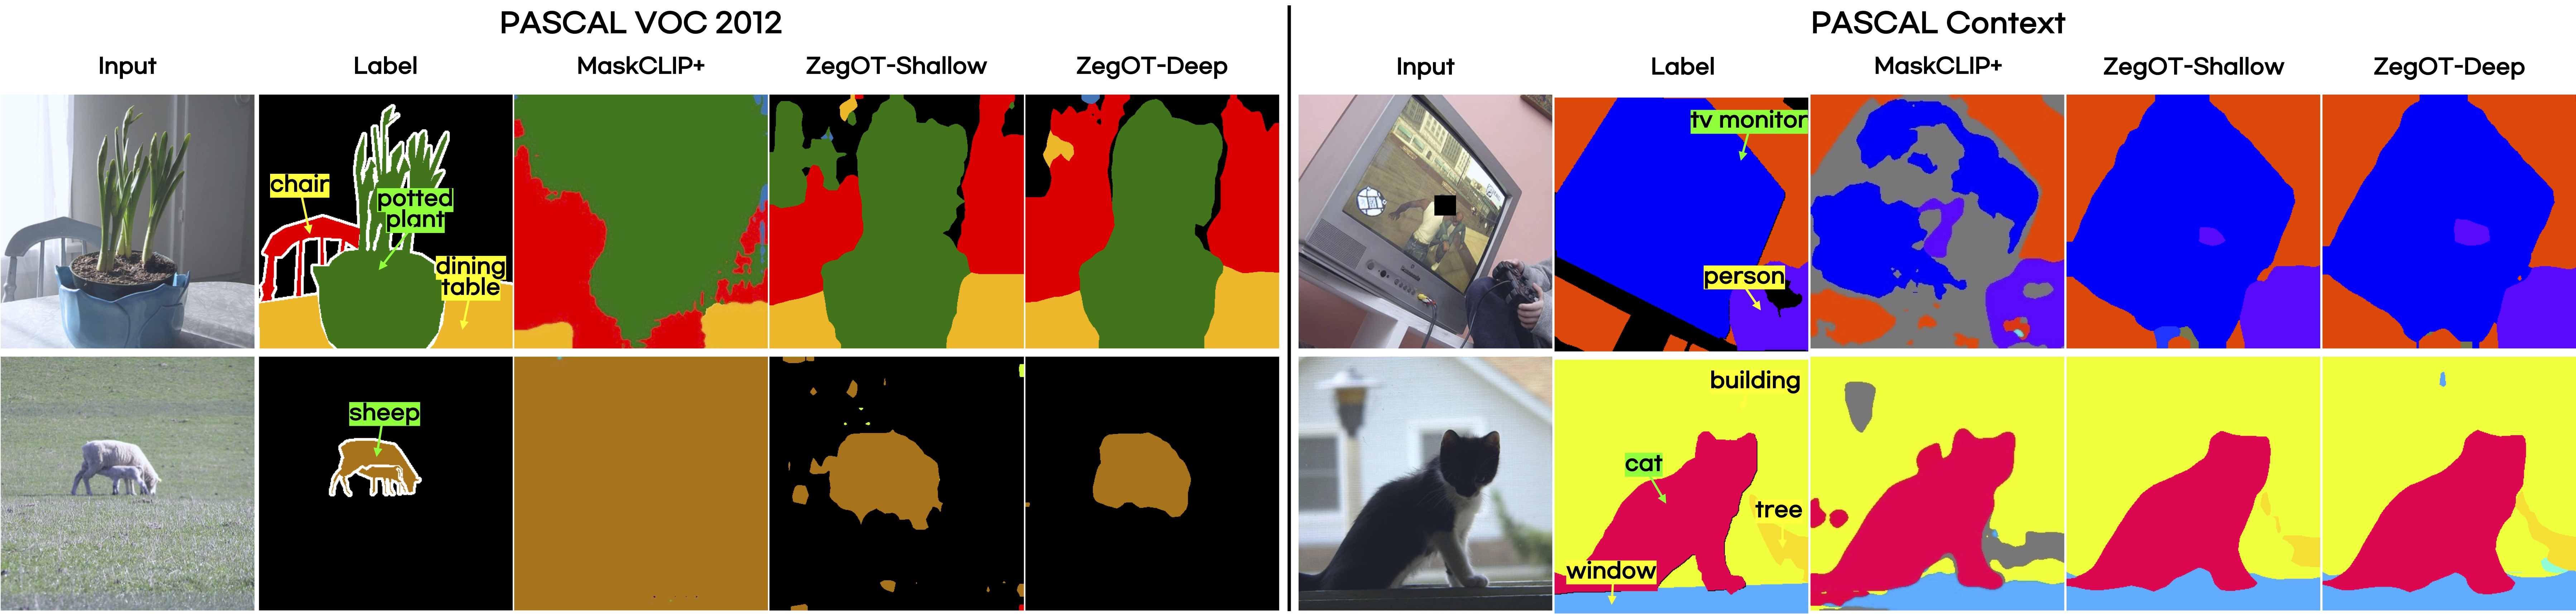
\includegraphics[width=0.95\linewidth]{fig/seg.jpg}
\caption{Qualitative zero-shot segmentation results on PASCAL VOC 2012 and PASCAL Context datasets. The  \colorbox{yellow}{yellow} tag indicates seen classes, while the \colorbox{green}{green} tag indicates unseen classes.}
\label{fig_seg}
\end{center}
\vskip -0.1in
\end{figure*}
%%%%%%%%%%%%%%%%%%%%%%%%%%%%%%%%%%%%%%%%%%%%%%%%%%%%%%%%%%%%%%%%%%%%%%%%%%%%%%%






\section{Experiments}

\subsection{Dataset and Evaluation Metric}
\paragraph{Dataset}
To evaluate the effectiveness of our proposed method, we carry out extensive experiments on three challenging datasets: PASCAL VOC 2012~\cite{everingham2012pascal}, PASCAL  Context~\cite{mottaghi2014role}, and COCO-Stuff164K~\cite{caesar2018coco}.  To fairly compare with previous methods~\cite{bucher2019zero,xu2021zsseg,ding2022zegformer,zhou2022maskclip,zhou2022zegclip}, we follow the identical protocol of dividing seen and unseen classes for each dataset. 
The dataset details are described in Appendix \ref{appen_datsset}.

% PASCAL VOC 2012 consists of 10,582 / 1,449 images with 20 categories, for training / validation. The dataset is divided into 15 seen and 5 unseen classes. PASCAL Context is an extensive dataset of PASCAL VOC 2010 that contains 4,996 / 5,104 images for training / test with 60 categories. The dataset is categorized into 50 seen and 10 unseen classes. COCO-Stuff 164K is a large-scale dataset that consists of 118,287 / 5,000 images for training / validation with 171 classes. The dataset is categorized into 156 seen and 15 unseen classes. 
\vspace{-0.2em}
\paragraph{Evaluation Metric}
By following previous works, we measure the mean of class-wise intersection over union (mIoU) on both seen and unseen classes, indicated as mIoU(S) and mIoU(U), respectively. We adopt the harmonic mean IoU (hIoU) of seen classes and unseen classes as a major metric. More details of the definition are deferred to Appendix~\ref{appendix:hIoU}. We also report the pixel-wise classification accuracy (pAcc) in Appendix~\ref{appendix:pAcc}. 

%\footnote{\url{https://github.com/open-mmlab/mmsegmentation}}
%\footnote{\url{https://github.com/openai/CLIP}}
\subsection{Implementation Details}
We implement the proposed method on the open-source toolbox MMSegmentation\footnote{\url{https://github.com/open-mmlab/mmsegmentation}} code base and conducted it on 4 RTX-3090 GPUs with batch size of 16.
We adopt the pre-trained CLIP ViT-B/16 model\footnote{\url{https://github.com/openai/CLIP}} as the frozen encoder module and adopt FPN which is equipped with atrous spatial pyramid pooling (ASPP) module as the image decoder for all the experiments.
Further details are deferred to Appendix \ref{appendix:implement}. We will release our source code for reproduction.
%In the first 1/10 training iterations, the model is trained on seen classes and we choose pseudo-label guided learning until reaching the first half of training iterations. The rest of the iterations adopt self-training.  


%%%%%%%%%%%%%%%%%%%%%%%%%%%%%%%%%%%%%%%%%%%%%%%%%%%%%%%%%%%%%%%%%%%%%%%%%%%%%%%
%% Scoremap Figure

\begin{figure*}[!t]
\vskip 0.1in
\begin{center}
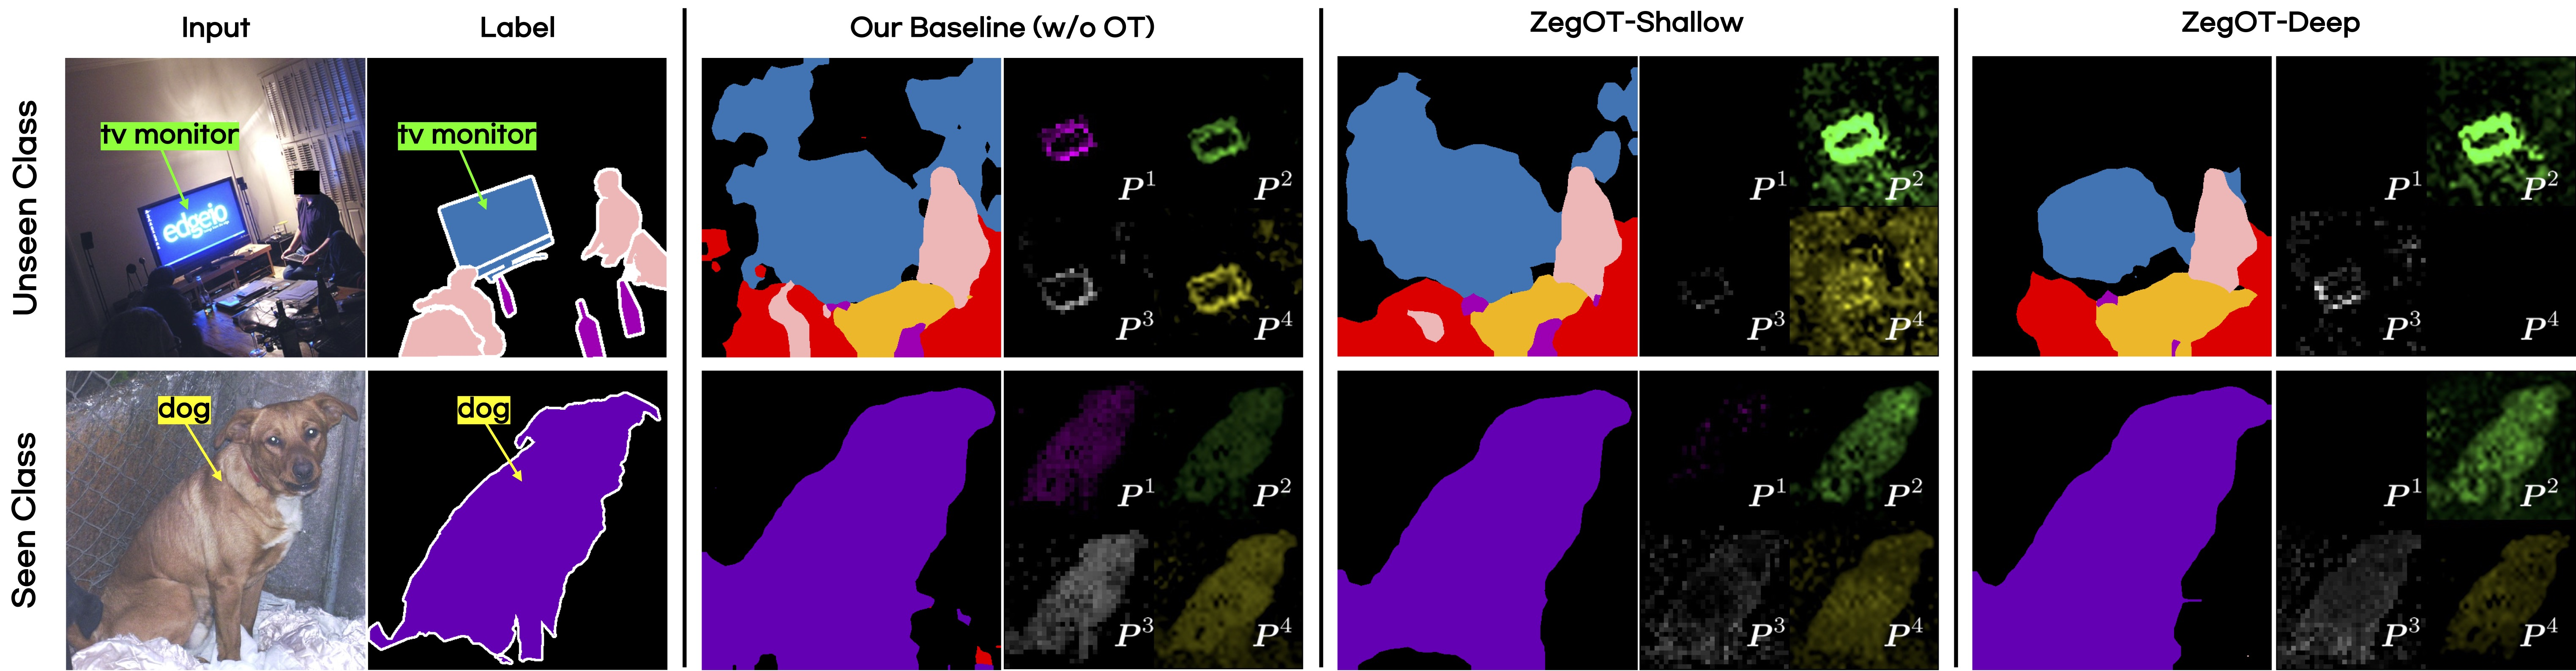
\includegraphics[width=0.95\linewidth]{fig/scoremap.jpg}
\caption{Visualization of the learned text prompt and image pixel alignment. For each method, we present its segmentation result (left) and $N$ multiple text prompts-related score matrix activated by the predicted class (right). In the baseline method without OT, all the $\bs{P}^i$-related score matrices resemble each others. On the other hand, our ZegOT-Shallow and ZegOT-Deep show separate score matrices, with ZegOT-Deep more focusing on different semantic attributes of the predicted class object.
}
\label{fig_main}
\end{center}
\vskip -0.1in
\end{figure*}
%%%%%%%%%%%%%%%%%%%%%%%%%%%%%%%%%%%%%%%%%%%%%%%%%%%%%%%%%%%%%%%%%%%%%%%%%%%%%%%

\subsection{Experimental Results}

\paragraph{Zero-shot Semantic Segmentation}
Figure ~\ref{fig_seg} shows the qualitative zero-shot segmentation performance of our ZegOT and the baseline method. Among the transductive methods, our ZegOT-Deep segments semantic objects most accurately on both PASCAL VOC and PASCAL Context datasets. Specifically, both our ZegOT-Shallow and ZegOT-Deep show superior performance on sectioning semantic boundaries of unseen objects compared to MaskCLIP+.
Quantitative results are also presented in Table~\ref{tab_main}. Our ZegOT-Deep achieves the SOTA performance for most datasets. 
For the largest COCO-Stuff-164K dataset, our ZegOT produces comparable qualitative segmentation results compared to the previous SOTA methods, as shown in Figure ~\ref{fig_seg_appen} of Appendix~\ref{appen_fig}. The drop in quantitative performance  in Table~\ref{tab_main} for this dataset  is because, compared to the retraining/fine-tuning methods, our current lightweight decoder with limited trainable parameters may be insufficient to be directly applied to the large-scale dataset. We expect this issue may be solved in a future study, by increasing the size of trainable model parameters. % and segmentation performance on a complex dataset.

\vspace{-0.5em}
\paragraph{OT-driven Text Prompt-Image Alignment}
To explore the origin of the superior segmentation performance of our ZegOT-Deep, we further analyze our proposed multi-prompt OT solver by visualizing each text prompt-related score matrix in Figure~\ref{fig_main}. For comparison, we set a multi-prompt baseline which basically shares ZegOT structure but the OT solver module is ablated. In the baseline method, all the text prompts $\mathcal{P}$-related score matrices  in Figure~\ref{fig_main} strikingly resemble each others, which implies that the multiple text prompts are converged to learn similar semantics. On the other hand, in ZegOT-Shallow, the multiple text prompts focus on different attributes of the target object, archieving fine-grained text-pixel alignment. However, a certain text prompt ($\bs{P}^4$ for each) tends to focus on background pixels rather than the foreground object. In ZegOT-Deep, each text prompt not only attends to different attributes, but a certain text prompt  ($\bs{P}^2$ for each) effectively highlights boundaries of the target object, which suggests that the model takes advantage of all the learned text prompts for improving segmentation performance. {Additional visualization of the text prompts-driven score matrices are provided in Figure~\ref{fig_score_appen} of Appendix~\ref{appen_fig}.}


\vspace{-0.2em}
\paragraph{Analysis on Deep Text Feature Alignment}
To demonstrate the effectiveness of the proposed DLFA, we conduct in-depth analysis comparing the strength of feature alignment with or without DLFA on PASCAL VOC 2012 dataset.
Figure~\ref{DLFA} shows the bar plot of average text-pixel alignment given a specific class name over the image encoder layer index.
To calculate the strength of feature alignment, we extract the score matrices $\{\bs{\hat S}_i|_{i=1}^{L}\}$ for a certain class name (\textit{e.g.}, dog) from the trained model and calculate the average $\bs{\hat S}_i$ along entire pixels for each image encoder layer.
We find that the strength of feature alignment with DLFA is much higher compared to that computed through the model without DLFA in almost layers. 
In particular, the average value of text-pixel alignment significantly increases at the earlier layers and the final layer. The result confirms that our model with DLFA effectively exploits the activated alignment between the two language-text modalities.


%%%%%%%%%%%%%%%%%%%%%%%%%%%%%%%%%%%%%%%%%%%%%%%%%%%%%%%%%%%%%%%%%%%%%%%%%%%%%%%
%%DLFA fIGURE
\begin{figure}[t]
\vskip 0.1in
\begin{center}
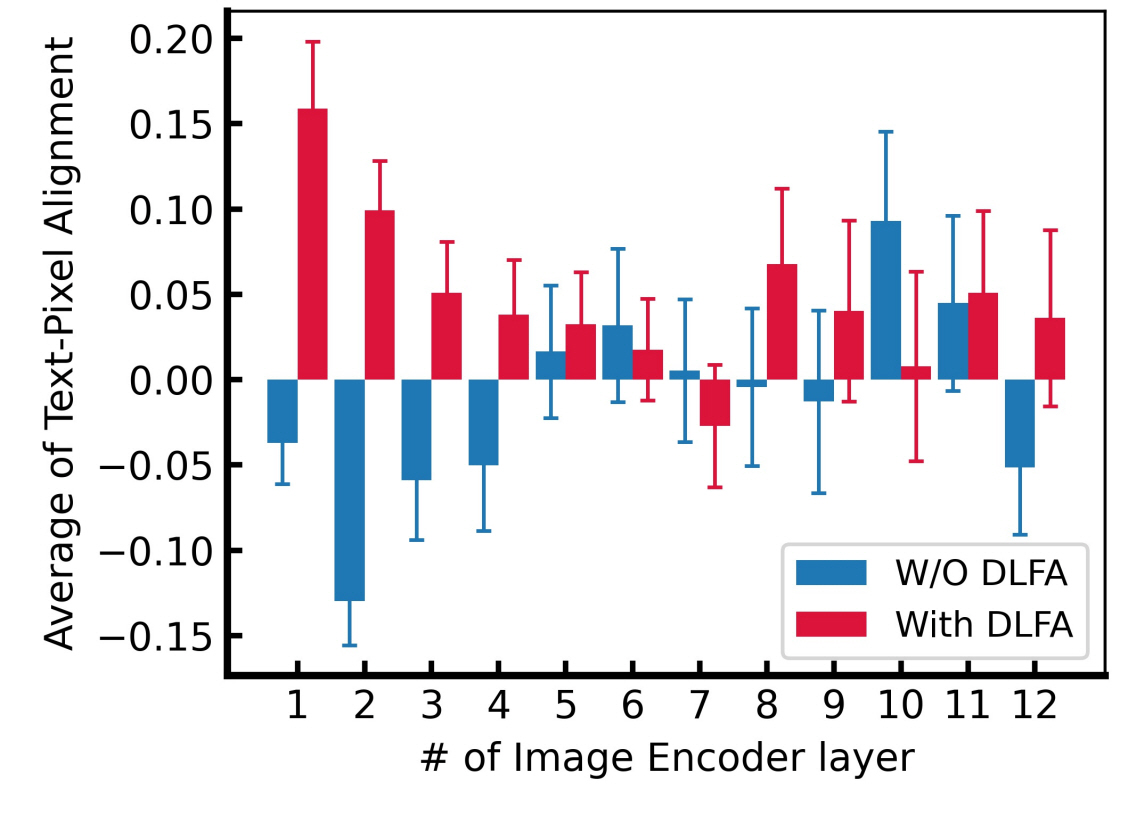
\includegraphics[width=0.8\linewidth]{fig/DLFA_2.jpg}
 \vspace{-0.35cm}
\caption{Bar plots of the average pixel-text alignment versus the image encoder layer index given a specific class name with or without Deep Local Feature Alignment (DLFA).}
\label{fig_dlfa}
\label{DLFA}
\end{center}
\vskip -0.1in
\end{figure}
%%%%%%%%%%%%%%%%%%%%%%%%%%%%%%%%%%%%%%%%%%%%%%%%%%%%%%%%%%%%%%%%%%%%%%%%%%%%%%%


\subsection{Ablation Studies}
%\paragraph{A. Effect of Multi Prompt OT solver}
\paragraph{Network Module Analysis}
To demonstrate the effectiveness of our proposed DLFA and MPOT modules, we further conduct ablation studies on PASCAL VOC 2012 dataset as reported in Table~\ref{tab:ablation}.  
Firstly, our baseline method without the DLFA module shows a drastic drop in performance on the unseen class, with a margin of -16.9$\%$ and -10.2$\%$ for each mIoU(U) and hIoU. The result suggests that our DLFA module efficiently transfers pre-trained CLIP knowledge to the deep local features to yield better text-pixel alignment under the ZS3 setting.
Next, we study the effect of the MPOT solver variants. In general, we observe that our MPOT brings improvement on unseen classes, while performances on seen classes are comparable throughout the entire method. Our ZegOT-Shallow outperforms the baseline by a margin of +1.9$\%$ and +1.0$\%$ for mIoU(U) and hIoU, respectively. 
Moreover, our ZegOT-Deep boosts the unseen performance by mIoU +6.2$\%$ and harmonic IoU +3.2$\%$ compared to the baseline, and these results are even comparable to the results of Oracle which is trained in a fully supervised manner. %The performance improvement may come from the optimally aligned score matrix of the learned text prompts and the frozen image features.
We confirm that the proposed structure with optimal transport framework certainly takes advantage of improving performance under the ZS3 setting.



%%%%%%%%%%%%%%%%%%%%%%%%%%%%%%%%%%%%%%%%%%%%%%%%%%%%%%%%%%%%%%%%%%%%%%%%%%%%%%%
%% Ablation Table
\begin{table}[t!]
\caption{Analysis of network module contribution.}
\label{tab:ablation}
\vskip 0.1in
\begin{center}
\resizebox{0.95\linewidth}{!}{
\begin{tabular}{lcccll}

\toprule
%\multirow{2}{*}{Model} & MPOT & Unseen & \multirow{2}{*}{mIoU(S)} & \multirow{2}{*}{mIoU(U)} & \multirow{2}{*}{hIoU}  \\
Model& DLFA &MPOT  & mIoU(S) &mIoU(U)  & hIoU\\
\cmidrule(r){1-1} \cmidrule(r){2-3} \cmidrule(r){4-5} \cmidrule(l){6-6}
%\midrule
\multirow{2}{*}{\textbf{Baseline}} 
 & \xmark &\xmark & 91.3 & 68.5\color{blue}{(-16.9)} & 78.3\color{blue}{(-10.2)}  \\
 & \cmark&\xmark & \textbf{91.9} & 85.4 & 88.5  \\
\cmidrule(r){1-1} \cmidrule(r){2-3} \cmidrule(r){4-5} \cmidrule(l){6-6}

\textbf{ZegOT-Shallow} & \cmark& Shallow & 91.8 & 87.3\color{red}{(+1.9)} & 89.5\color{red}{(+1.0)}  \\

\textbf{ZegOT-Deep} & \cmark &Deep & 91.9 & \textbf{91.6}\color{red}{(+6.2)} & \textbf{91.7}\color{red}{(+3.2)}  \\

\cmidrule(r){1-1} \cmidrule(r){2-3} \cmidrule(r){4-5} \cmidrule(l){6-6}
\textbf{Oracle} & \cmark& Deep &  92.0 & 91.6 & 91.8 \\
\bottomrule

\end{tabular}
}
\end{center}
\vskip -0.1in
\end{table}
%%%%%%%%%%%%%%%%%%%%%%%%%%%%%%%%%%%%%%%%%%%%%%%%%%%%%%%%%%%%%%%%%%%%%%%%%%%%%%%


%%%%%%%%%%%%%%%%%%%%%%%%%%%%%%%%%%%%%%%%%%%%%%%%%%%%%%%%%%%%%%%%%%%%%%%%%%%%%%%
%% Component Analysis Table

\begin{table}[!t]
\caption{Component analysis of hyper-parameters. $\#$ denotes the hyper-parameters of configurations. Checkmark $\checkmark$ indicates the default configuration of ZegOT-Shallow and ZegOT-Deep.}
\label{tab:Component}
\vskip 0.1in
\begin{center}
\resizebox{0.95\linewidth}{!}{
\begin{tabular}{lccccc}

\toprule
%\multicolumn{2}{c|}
Components & $\#$ &mIoU (S) & mIoU (U) & hIoU & ZegOT \\

\cmidrule(r){1-1} \cmidrule(l){2-2} \cmidrule(l){3-5}  \cmidrule(l){6-6}
\multirow{3}{*}{Number of text prompts} & 2 & 91.6& 82.9 & 87.0 \\
& 4 & \bf{91.9}& \bf{91.6} & \bf{91.7} & \checkmark\\
& 6 & 91.8& 89.6 & 90.7 \\
\cmidrule(r){1-1} \cmidrule(l){2-2} \cmidrule(l){3-5}  \cmidrule(l){6-6}
\multirow{5}{*}{Depth of MPOT} & 12 & 91.8& 87.3 & 89.5 & \checkmark-Shallow \\
& 10-12 & 91.4& 87.3& 89.3\\
& 8-12 & 91.9& \bf{91.6}& \bf{91.7}& \checkmark-Deep \\
& 4-12 & 91.6& 90.2& 90.9 \\
& 1-12 & \bf{92.1} & 86.5 & 89.3 &\\
\bottomrule
\end{tabular}
}
\end{center}
\vskip -0.1in
\end{table}
%%%%%%%%%%%%%%%%%%%%%%%%%%%%%%%%%%%%%%%%%%%%%%%%%%%%%%%%%%%%%%%%%%%%%%%%%%%%%%%


% \paragraph{B. Effect of Hyper-parameter of Components}
\paragraph{Effect of Hyper-parameters of Network Components}
To further investigate the effect of components that consist our network, we conduct the component analysis on hyper-parameter as shown in Table~\ref{tab:Component}.
%\subparagraph{Number of Text Prompts} 
%We perform an ablation study on the number of text prompts $N$. 
Firstly, we observe the segmentation performance by varying the total number $N$ of the learnable text prompts.
%When $N$=4, ZegOT performs the best, which indicates that fewer text prompts ($N$=2) can not learn comprehensive semantic features and larger $N$ ($N$=6) results in too complicated for optimal transport matching.    
We empirically find that ZegOT performs the best when $N=4$, but the performance drops when $N$ is decreased to $2$ or increased to $6$, which implies that fewer text prompts are insufficient to learn comprehensive semantic features, whereas too many text prompts complicate the optimal transport matching process.
% \subparagraph{Depth of OT Solver}  %Layers for inserting OT Solver
%We carry out the experiment to explore the effect of depth for inserting OT solver in different layers. 
We further explore the effect of the depth of MPOT solver, $\textit{i.e.,}$ ranges of the frozen image encoder layers that inserted to MPOT.
Although inserting multiple layers to MPOT boosts performance, 
it also causes performance trade-off between seen and unseen classes segmentation.
We find that introducing the MPOT with 8 to 12-th layers of the image encoder achieves the best performance, which becomes % which is 
the default setting of ZegOT-Deep for the entire experiments.

%%%%%%%%%%%%%%%%%%%%%%%%%%%%%%%%%%%%%%%%%%%%%%%%%%%%%%%%%%%%%%%%%%%%%%%%%%%%%%%
%%%%%%%%%%%%%%%%%%%%%%%%%%%%%%%%%%%%%%%%%%%%%%%%%%%%%%%%%%%%%%%%%%%%%%%%%%%%%%%
\section{Conclusion}
In this work, we proposed ZegOT, a cost-effective segmentation framework that optimizes multiple text prompts by utilizing a frozen visual-language model, which thoroughly leverages the aligned vision and language knowledge for zero-shot semantic segmentation tasks. 
We also incorporated optimal transport theory into our framework to train multiple text prompts for representing different semantic properties. 
We demonstrated that our Zeg-OT outperforms the state-of-the-art zero-shot semantic segmentation approaches on various benchmark datasets with the lightest model parameters. 
Our in-depth analyses also confirmed that our ZegOT effectively delivers performance gains on both seen and unseen classes. \footnote{Limitations and negative impacts are deferred to Appendix~\ref{appen_limit}.}




%%%%%%%%%%%%%%%%%%%%%%%%%%%%%%%%%%%%%%%%%%%%%%%%%%%%%%%%%%%%%%%%%%%%%%%%%%%%%%%
%%%%%%%%%%%%%%%%%%%%%%%%%%%%%%%%%%%%%%%%%%%%%%%%%%%%%%%%%%%%%%%%%%%%%%%%%%%%%%%
% Acknowledgements should only appear in the accepted version.
% \section*{Acknowledgements}

% \textbf{Do not} include acknowledgements in the initial version of
% the paper submitted for blind review.



%%%%%%%%%%%%%%%%%%%%%%%%%%%%%%%%%%%%%%%%%%%%%%%%%%%%%%%%%%%%%%%%%%%%%%%%%%%%%%%
%%%%%%%%%%%%%%%%%%%%%%%%%%%%%%%%%%%%%%%%%%%%%%%%%%%%%%%%%%%%%%%%%%%%%%%%%%%%%%%
% References

\newpage

\bibliography{icml2023_zegot}
\bibliographystyle{icml2023}





%%%%%%%%%%%%%%%%%%%%%%%%%%%%%%%%%%%%%%%%%%%%%%%%%%%%%%%%%%%%%%%%%%%%%%%%%%%%%%%
%%%%%%%%%%%%%%%%%%%%%%%%%%%%%%%%%%%%%%%%%%%%%%%%%%%%%%%%%%%%%%%%%%%%%%%%%%%%%%%
% APPENDIX

\clearpage
\newpage
\newpage

\appendix

\begin{table*}[h]
	\caption{Notation of the baseline and our proposed method}
	\label{tab:notation}
	\vskip 0.1in
	\begin{center}
		\resizebox{0.8\linewidth}{!}{
			\begin{tabular}{lccccc}
				
				\toprule
				%\multirow{2}{*}{Model} & MPOT & Unseen & \multirow{2}{*}{mIoU(S)} & \multirow{2}{*}{mIoU(U)} & \multirow{2}{*}{hIoU}  \\
				Model& DLFA &MPOT  & Decoder Output & Intermediate Score maps  & Final Score map\\
				\cmidrule(r){1-1} \cmidrule(r){2-3} \cmidrule(r){4-5} \cmidrule(l){6-6}
				%\midrule
				\multirow{2}{*}{\textbf{Baseline}} 
				& \xmark &\xmark & $\mathbf{Y}$ & $\{\bs{S}_i\}^L_{i=1}$ & $\bs{S}_L$ \\
				& \cmark&\xmark & $\mathbf{\hat Y}$ & $\{\bs{\hat S}_i\}^L_{i=1}$ & $\bs{\hat S}_L$  \\
				\cmidrule(r){1-1} \cmidrule(r){2-3} \cmidrule(r){4-5} \cmidrule(l){6-6}
				
				\textbf{ZegOT-Shallow} & \cmark& Shallow & $\asty$ &  $\{\bs{\hat S}_i\}^L_{i=1}$ & $\bs{S}^*_L$ in \eqref{eq:shallow} \\
				
				\textbf{ZegOT-Deep} & \cmark &Deep & $\asty$ &  $\{\bs{\hat S}_i\}^L_{i=1}$ & $\bs{S}^*_L$ in \eqref{eq:deep}  \\
				\bottomrule
				
			\end{tabular}
		}
	\end{center}
	\vskip -0.1in
\end{table*}

\section{Limitations and Negative Societal Impacts}
\label{appen_limit}
\paragraph{Limitations}
Our model performance is highly dependent on the CLIP model knowledge. Specially, the class name-driven unseen object segmentation can be failed, unless the CLIP model is pre-trained with the target class-related image-text pairs.


\paragraph{Negative Societal Impacts}
Our paper has a potential privacy issue in providing visual results of the person class. To avoid the issue, every person in all the figures are properly anonymized by covering the faces.



\section{Notation} \label{apppendix:notation}
We provide a summary of notation in Table \ref{tab:notation}





\section{Zero-shot Segmentation Training Process.} \label{sec_phase}

By following the general transductive zero-shot semantic segmentation (ZS3) setting \cite{pastore2021strict, zhou2022maskclip, zhou2022zegclip}, we divide the entire training procedure into 3 phases, 
and the label $\gty$ is phase-adaptively altered for training the unseen classes, as described in Algorithm \ref{algoritm_phases1}.


%%%%%%%%%%%%%%%%%%%%%%%%%%%%%%%%%%%%%%%%%%%%%%%%%%%%%%%%%%%%%%%%%%%%%%%%%%%%%%%
%%Training Phase
\begin{algorithm}
\caption{ZegOT Pseudo-code}\label{algoritm_phases1}
\label{alg:phase1}
{\bfseries Input:} ZegOT model $Z_t$ at iteration $t$, The subset of seen classes $\mc{C}_S$ and unseen classes $\mc{C}_U$, $\textit{e.g,}$ $\mc{C}_S \cap \mc{C}_U = \emptyset$. The training dataset $D = \{(x,\gty)| x \in \mathcal{X}, \gty_{hw}\in \mc{C}_S\}$, the iteration of seen class-guided learning $T_g$, the iteration of pseudo-guided learning $T_{p}$, self-trianing iterations $T_s$, upsampling operator $\mathcal{R}_{u}$, downsampling operator $\mathcal{R}_{d}$;\\ 
{\bfseries Phase 1: Seen class-guided learning}\\
\For{$t=1, 2, \cdots, T_g$ }{
	$\asty, \bs{S^{\ast}} \leftarrow$ model prediction from $Z_{t}(x)$;\\
	% $ \mathcal{L} \leftarrow \lambda_{\text{seg}}\mathcal{L}_{seg}(\hat y, y) + \lambda_{\text{score}} \mathcal{L}_{score}(\bs{S^{\ast}}, \textit{Down}(y))$; \\
    $\mathcal{L}_{} \leftarrow \lambda_{\text{seg}}\mathcal{L}_{\text{seg}}(\asty, \gty)\\ 
    {} \quad + \lambda_{\text{score}} \mathcal{L}_{\text{score}}(\mathcal{M}(\bs{S}^{\ast}_L),\mathcal{R}_{d}(\gty))$;
    \\
    $Z_{t+1}\leftarrow$ AdamW model parameter update;}

{\bfseries Phase 2: Pseudo-guided learning};\\
\For{$x,y$ in $D$}{
	\If{$\gty_{hw} \not\in \mc{C}_S$} %Unseen label이 없다고 가정해야 하기 때문에 $C_S$가 아닐때로 바꾸겠습니당
	{$\gty_{hw} = \underset{\bs{c} \in \mc{C}_U}{\arg{\max}} \ Z_{T_g}(\mathcal{R}_{u}(\mathcal{M}(\bs{S^{\ast}}))_{hw} = \bs{c}|x)$;}
	}
\For{$t=T_g +1,T_g + 2, \cdots, T_{p}$}
{$\asty, \bs{S^{\ast}} \leftarrow$ model prediction from $Z_{t}(x)$; \\
$\mathcal{L} \leftarrow \lambda_{\text{seg}}\mathcal{L}_{\text{seg}}(\asty, \gty)\\ 
    {} \quad + \lambda_{\text{score}} \mathcal{L}_{\text{score}}(\mathcal{M}(\bs{S}^{\ast}_L),\mathcal{R}_{d}(\gty))$;
% $ \mathcal{L} \leftarrow \lambda_{\text{seg}}\mathcal{L}_{seg}(\asty, \gty) + \lambda_{\text{score}} \mathcal{L}_{score}(\bs{S^{\ast}}, \mathcal{R}_{d}(y))$; \\
\\
$Z_{t+1}\leftarrow$ AdamW model parameter update;}
	
{\bfseries Phase 3: Self-training}

\For{$t=T_{p} +1,T_{p} + 2, \cdots, T_{p}+T_s$}
{
$\asty, \bs{S^{\ast}} \leftarrow$ model prediction from $Z_{t}(x)$; \\
\If{$\gty_{hw} \not\in \mc{C}_S$}
{$\gty_{hw} = \underset{\bs{c} \in \mc{C}_U}{\arg{\max}} \ Z_{t-1}(\mathcal{R}_{u}(\mathcal{M}(\bs{S^{\ast}}))_{hw} = \bs{c}|x)$;}
$ \mathcal{L} \leftarrow \lambda_{\text{seg}}\mathcal{L}_{seg}(\asty, \gty) \\ 
    {} \quad +\lambda_{\text{score}} \mathcal{L}_{\text{score}}(\mathcal{M}(\bs{S}^{\ast}_L),\mathcal{R}_{d}(\gty))$; \\
$Z_{t+1}\leftarrow$ AdamW model parameter update;
}   
\end{algorithm}
%%%%%%%%%%%%%%%%%%%%%%%%%%%%%%%%%%%%%%%%%%%%%%%%%%%%%%%%%%%%%%%%%%%%%%%%%%%%%%%


\paragraph{Phase 1. Seen Class Supervised Training}
For the first $1/10$ training iterations, the model is trained utilizing the ground truth label $\gty$, which only contains pixel-wise labels $\gty_{hw}$ for seen classes $\mc{C}_S$, and the rest labels are ignored for calculating losses. 

\paragraph{Phase 2. Unseen Class Pseudo-label Guided Training}
Once the network is trained, the learned knowledge can be transferred to update the labels for unseen classes $\mc{C}_U$. Since the learnable decoder is optimized for the seen class-only, we only utilize score matrix $\bs{S^{\ast}}$ for updating each pixel value of the ground truth label $\gty_{hw}$ which not belongs to $\mc{C}_S$, while keeping original labels for $\mc{C}_S$.
Then, the model is trained utilizing the updated pseudo-label, until reaching the half of the training iterations.

\paragraph{Phase 3. Unseen Class Self Training}
For the rest of the training iterations, the model self-generates each pixel values of the ground truth label $\gty_{hw}$ which not belongs to $\mc{C}_S$, at every training iteration.% The only difference compared to Phase 2 is that $\bs{S^{\ast}}$ is continuously updated.



\section{Optimal Transport algorithm} 
\label{algo-ot}
\begin{algorithm}
	\caption{Optimal Transport with Sinkhorn algorithm}
	\label{algo-2}
	\SetKwInOut{Input}{Input}
	\SetKwInOut{Output}{Output}
	\SetKwInput{kwInit}{Initialization}
	\SetKwInput{kwset}{Given}
	\kwset{$\bs{\mu} = \bs{1}^{M}/M$, $\bs{\nu} = \bs{1}^{N}/N$, the score matrix $\bs{\hat{S}}$ ;}
	\Input{The cost matrix $\bs{C} = \bs{1 - \hat S}$, hyper-paramter $\lambda$, the max iteration $t_{max}$;}
	\kwInit{$\bs{K} = \exp(-\bs{C}/\lambda)$, $t \leftarrow 1, \bs{b}^0 = 1$;}
	\While{$t \leq t_{max}$ \text{and not converge} }{
	$\bs{a}^t = \bs{\mu}$ / $(\bs{Kb}^{t-1})$; \\ 
	$\bs{b}^t = \bs{\nu}$ / $(\bs{K^{\top}a}^t)$;
	}
	\Output{Optimal transport plan $\bs{T}^{\ast}$ = $\text{diag}(\bs{a})^t\bs{K}\text{diag}(\bs{b})^t$ ;}
\end{algorithm}


\section{Details of Loss function}
\label{appendix:loss}
As discussed in Section~\ref{sec:loss}, we combine three different losses, including Cross Entropy (CE) loss, the focal loss based on Binary Cross Entropy (BCE) loss, and the dice loss, which are given  by:
\begin{align}
\begin{split}
\mathcal{L}_{\text{CE}} = -\frac{1}{HW} \sum^{HW}_{i=1} \gty_i \log(\phi(\asty_i)) \\
    + (1- \gty_i)\log(1-\phi(\asty_i)), \\   
\end{split}\\
\begin{split}
\mathcal{L}_{\text{focal}} = -\frac{1}{HW} \sum^{HW}_{i=1}\gty_i (1- \sigma(\asty_i))^{\gamma} \log(\sigma(\asty_i) )\\
    + (1- \gty_i)\sigma(\asty_i)^{\gamma}\log(1-\sigma(\asty_i)), \\   
\end{split}\\    
\begin{split}
\mathcal{L}_{\text{dice}} = 1 -\frac{2\sum^{HW}_{i=1}\gty_i \asty_i}{\sum^{HW}_{i=1} {\gty_i}^2 + \sum^{HW}_{i=1} {\asty_i}^2}, 
\end{split} \\
\end{align}
where $\asty$ is the model decoder outputs of the decoder, $\gty$ is the ground truth label, $\phi(\cdot)$ and $\sigma(\cdot)$ are Softmax and Sigmoid operations, for each, $\gamma$ is a hyper-parameter to balance hard and easy samples, which is set to 2.
Throughout the entire experiments,
$\lambda_{\text{CE}}, \lambda_{\text{focal}}$, and $\lambda_{\text{dice}}$ are set to 1, 20, and 1, respectively. In \eqref{seg,score_loss}, both $\lambda_{\text{seg}}$ and  $\lambda_{\text{score}}$ are set to 1. 
The above losses are for computing $\mathcal{L}_{\text{seg}}$ in \eqref{losses}, and when to compute $\mathcal{L}_{\text{score}}$, the input $\asty$ and the ground truth $\gty$ are replaced by $\mathcal{M}(\bs{S}^{\ast}_L)$ and $\mathcal{R}_{d}(\gty)$, respectively, where .



\section{Details of Dataset}
\label{appen_datsset}

We utilize a total of three datasets, $\textit{i.e.,}$ PASCAL VOC 2012~\cite{everingham2012pascal}, PASCAL  Context~\cite{mottaghi2014role}, and COCO-Stuff164K~\cite{caesar2018coco}. 
We divide seen and unseen classes for each dataset, following the settings of previous methods~\cite{bucher2019zero,xu2021zsseg,ding2022zegformer,zhou2022maskclip,zhou2022zegclip}. PASCAL VOC 2012 consists of 10,582 / 1,449 images with 20 categories, for training / validation. The dataset is divided into 15 seen and 5 unseen classes. PASCAL Context is an extensive dataset of PASCAL VOC 2010 that contains 4,996 / 5,104 images for training / test with 60 categories. The dataset is categorized into 50 seen and 10 unseen classes. COCO-Stuff 164K is a large-scale dataset that consists of 118,287 / 5,000 images for training / validation with 171 classes. The dataset is categorized into 156 seen and 15 unseen classes. 


%%%%%%%%%%%%%%%%%%%%%%%%%%%%%%%%%%%%%%%%%%%%%%%%%%%%%%%%%%%%%%%%%%%%%%%%%%%%%%%
% pACC

\begin{table}[h]
	\caption{Zero-shot semantic segmentation performance (pAcc).}
	\label{tab:Acc}
	\vskip 0.1in
	\begin{center}
		\resizebox{1\linewidth}{!}{
			\begin{tabular}{clcccr}
				
				\toprule
				\multirow{2}{*}{Settings} & \multirow{2}{*}{Method} & \multirow{2}{*}{\thead{PASCAL \\ VOC 2012}} & \multirow{2}{*}{\thead{PASCAL \\ Context}} & \multirow{2}{*}{\thead{COCO-Stuff \\ 164K}} & \multirow{2}{*}{\thead{\#Param}} \\
				&\\
				\cmidrule(r){1-1} \cmidrule(l){2-2} \cmidrule(l){3-5}  \cmidrule(l){6-6}
				\multirow{4}{*}{\thead{Inductive \\ (Seen supervised)}} & CaGNet & 80.7 & 59.2 & 56.6 & 101M\\
				& ZegFormer & - & - & - & 41M\\
				& zsseg & - & - & 60.3 & 61M\\
				& ZegCLIP & 94.6 & 76.2 & 62.0 & 130M \\
				\cmidrule(r){1-1} \cmidrule(l){2-2} \cmidrule(l){3-5}  \cmidrule(l){6-6}
				
				\multirow{7}{*}{\thead{Transductive \\ w/ Self Training \\ (Seen supervised + \\  Unseen self-supervised)}} & CaGNet & 81.6 & 59.6 & 56.8 & 101M \\
				& STRICT & - & - & - & 101M \\
				& zsseg & - & - & - & 61M \\
				& MaskCLIP+ & 94.0 & 74.8 & 67.6 & 140M \\
				& ZegCLIP & 95.1 & 77.2 & \textbf{68.8} & 130M \\
				& \textbf{ZegOT-Shallow} & 95.6 & \textbf{80.9} & 65.7 & \textbf{21M} \\
				& \textbf{ZegOT-Deep} & \textbf{96.0} & 80.8 & 64.2 & \textbf{21M} \\
				\bottomrule
				
			\end{tabular}
		}
	\end{center}
	\vskip -0.1in
\end{table}
%%%%%%%%%%%%%%%%%%%%%%%%%%%%%%%%%%%%%%%%%%%%%%%%%%%%%%%%%%%%%%%%%%%%%%%%%%%%%%%

%%%%%%%%%%%%%%%%%%%%%%%%%%%%%%%%%%%%%%%%%%%%%%%%%%%%%%%%%%%%%%%%%%%%%%%%%%%%%%%
% Componant analysis table

\begin{table}[h]
	\caption{Component analysis of hyper-parameter of our method. $\#$ denotes the hyper-parameters of configurations. Checkmark $\checkmark$ indicates that the default configuration of ZegOT.}
	\label{tab:Component2}
	\vskip 0.1in
	\begin{center}
		\resizebox{1\linewidth}{!}{
			\begin{tabular}{lccccc}
				
				\toprule
				Components & $\#$ & mIoU (S) & mIoU (U) & hIoU & ZegOT \\
				\cmidrule(r){1-1} \cmidrule(l){2-2} \cmidrule(l){3-5}  \cmidrule(l){6-6}
				\multirow{3}{*}{Context length ($l$)} & 8 & 91.9& \bf{91.6}& \bf{91.7}& \checkmark \\
				& 16 & \bf{92.2}& 89.6& 90.9\\
				& 32 & 91.9& 90.3& 91.1\\
				\cmidrule(r){1-1} \cmidrule(l){2-2} \cmidrule(l){3-5}  \cmidrule(l){6-6}
				\multirow{5}{*}{Score matrix weight ($w$)} & 0.6 & 91.0 & 91.4& 91.2 & \\
				& 0.7 &  91.0 & 91.5 & 91.3  & \\
				& 0.8 &  \bf{91.9}& 91.6& \bf{91.7} & \checkmark \\
				& 0.9 &  91.5 & \bf{91.7} & 91.6&  \\
				& 1.0 & 89.5 & 88.4 & 88.9&\\
				\bottomrule
			\end{tabular}
		}
	\end{center}
	\vskip -0.1in
\end{table}



\section{Implementation Detail}
\label{appendix:implement}
 We further declare the implementation detail for our work. 
 Input image resolution is set as 480$\times$480 for PASCAL Context, and 512$\times$512 for the rest of the datasets. The context length is set to 8 and the weight $w$ for the score matrix~\eqref{eq:final_predict} is set to 0.8. We choose the lightest training schedule, which is 20K / 40K / 80K for PASCAL VOC 2012 / PASCAL Context / COCO-Stuff-164K. 



\section{Definition of Harmonic mean IoU}
\label{appendix:hIoU}
Following the previous works ~\cite{xu2021zsseg,zhou2022maskclip,zhou2022zegclip}, we define harmonic mean IoU (hIoU) among the seen and unseen classes as:
\begin{align}
    \text{hIoU} =\frac{2 * \text{mIoU(S) +mIoU(U)}}{\text{mIoU(S)+mIoU(U)}}
\end{align}


\section{Quantitative Analysis on Zero-Shot Segmentation Performance}
\label{appendix:pAcc}
We further report pixel-wise classification accuracy (pAcc) compared to baseline methods similar with Table~\ref{tab_main}.


\section{Further Analysis on Hyper-parameters.}
\label{appendix:compo}
Similar to Table~\ref{tab:Component}, we further conduct the component analysis with varying hyper-parameters including: context length ($l$), and score matrix weight $(w)$.
Firstly, we empirically find that the large context length is limited to take %\textbf{}
significant effect on segmentation performance, \textit{e.g,} when $l=16$, the performance on seen classes is the best, but the performance on unseen classes drops. Since we consider the hIoU as a major metric, we adopt $l=8$ as the default setting. 

We further investigate the effect of the score matrix 
weight, which is described in Eq.~\eqref{eq:final_predict} for the network inference.
We observe that ZegOT performs the best when $w = 0.8$, but the performance gradually drops when $w$ is further decreased or increased. In addition, we find that the segmentation performance on both seen and unseen classes significantly drops when $w=1.0$, which means that $\hat y$ is also important to predict the final segmentation maps. 



%%%%%%%%%%%%%%%%%%%%%%%%%%%%%%%%%%%%%%%%%%%%%%%%%%%%%%%%%%%%%%%%%%%%%%%%%%%%%%%





\section{Additional Visual Results.}
\label{appen_fig}
We provide additional visual results. Figure~\ref{fig_seg_appen} and Figure~\ref{fig_seg_appen2} show
qualitative zero-shot segmentation performance of our ZegOT and the baseline method for COCO-Stuff164K, PASCAL VOC 2012 and PASCAL Context datasets. 
Figure~\ref{fig_score_appen} shows additional visual results of text prompt-related score matrix on PASCAL VOC 2012 dataset.


\pagebreak

%%%%%%%%%%%%%%%%%%%%%%%%%%%%%%%%%%%%%%%%%%%%%%%%%%%%%%%%%%%%%%%%%%%%%%%%%%%%%%%
%% Segmentation comparison COCO

\begin{figure*}[!t]
\vskip 0.1in
\begin{center}
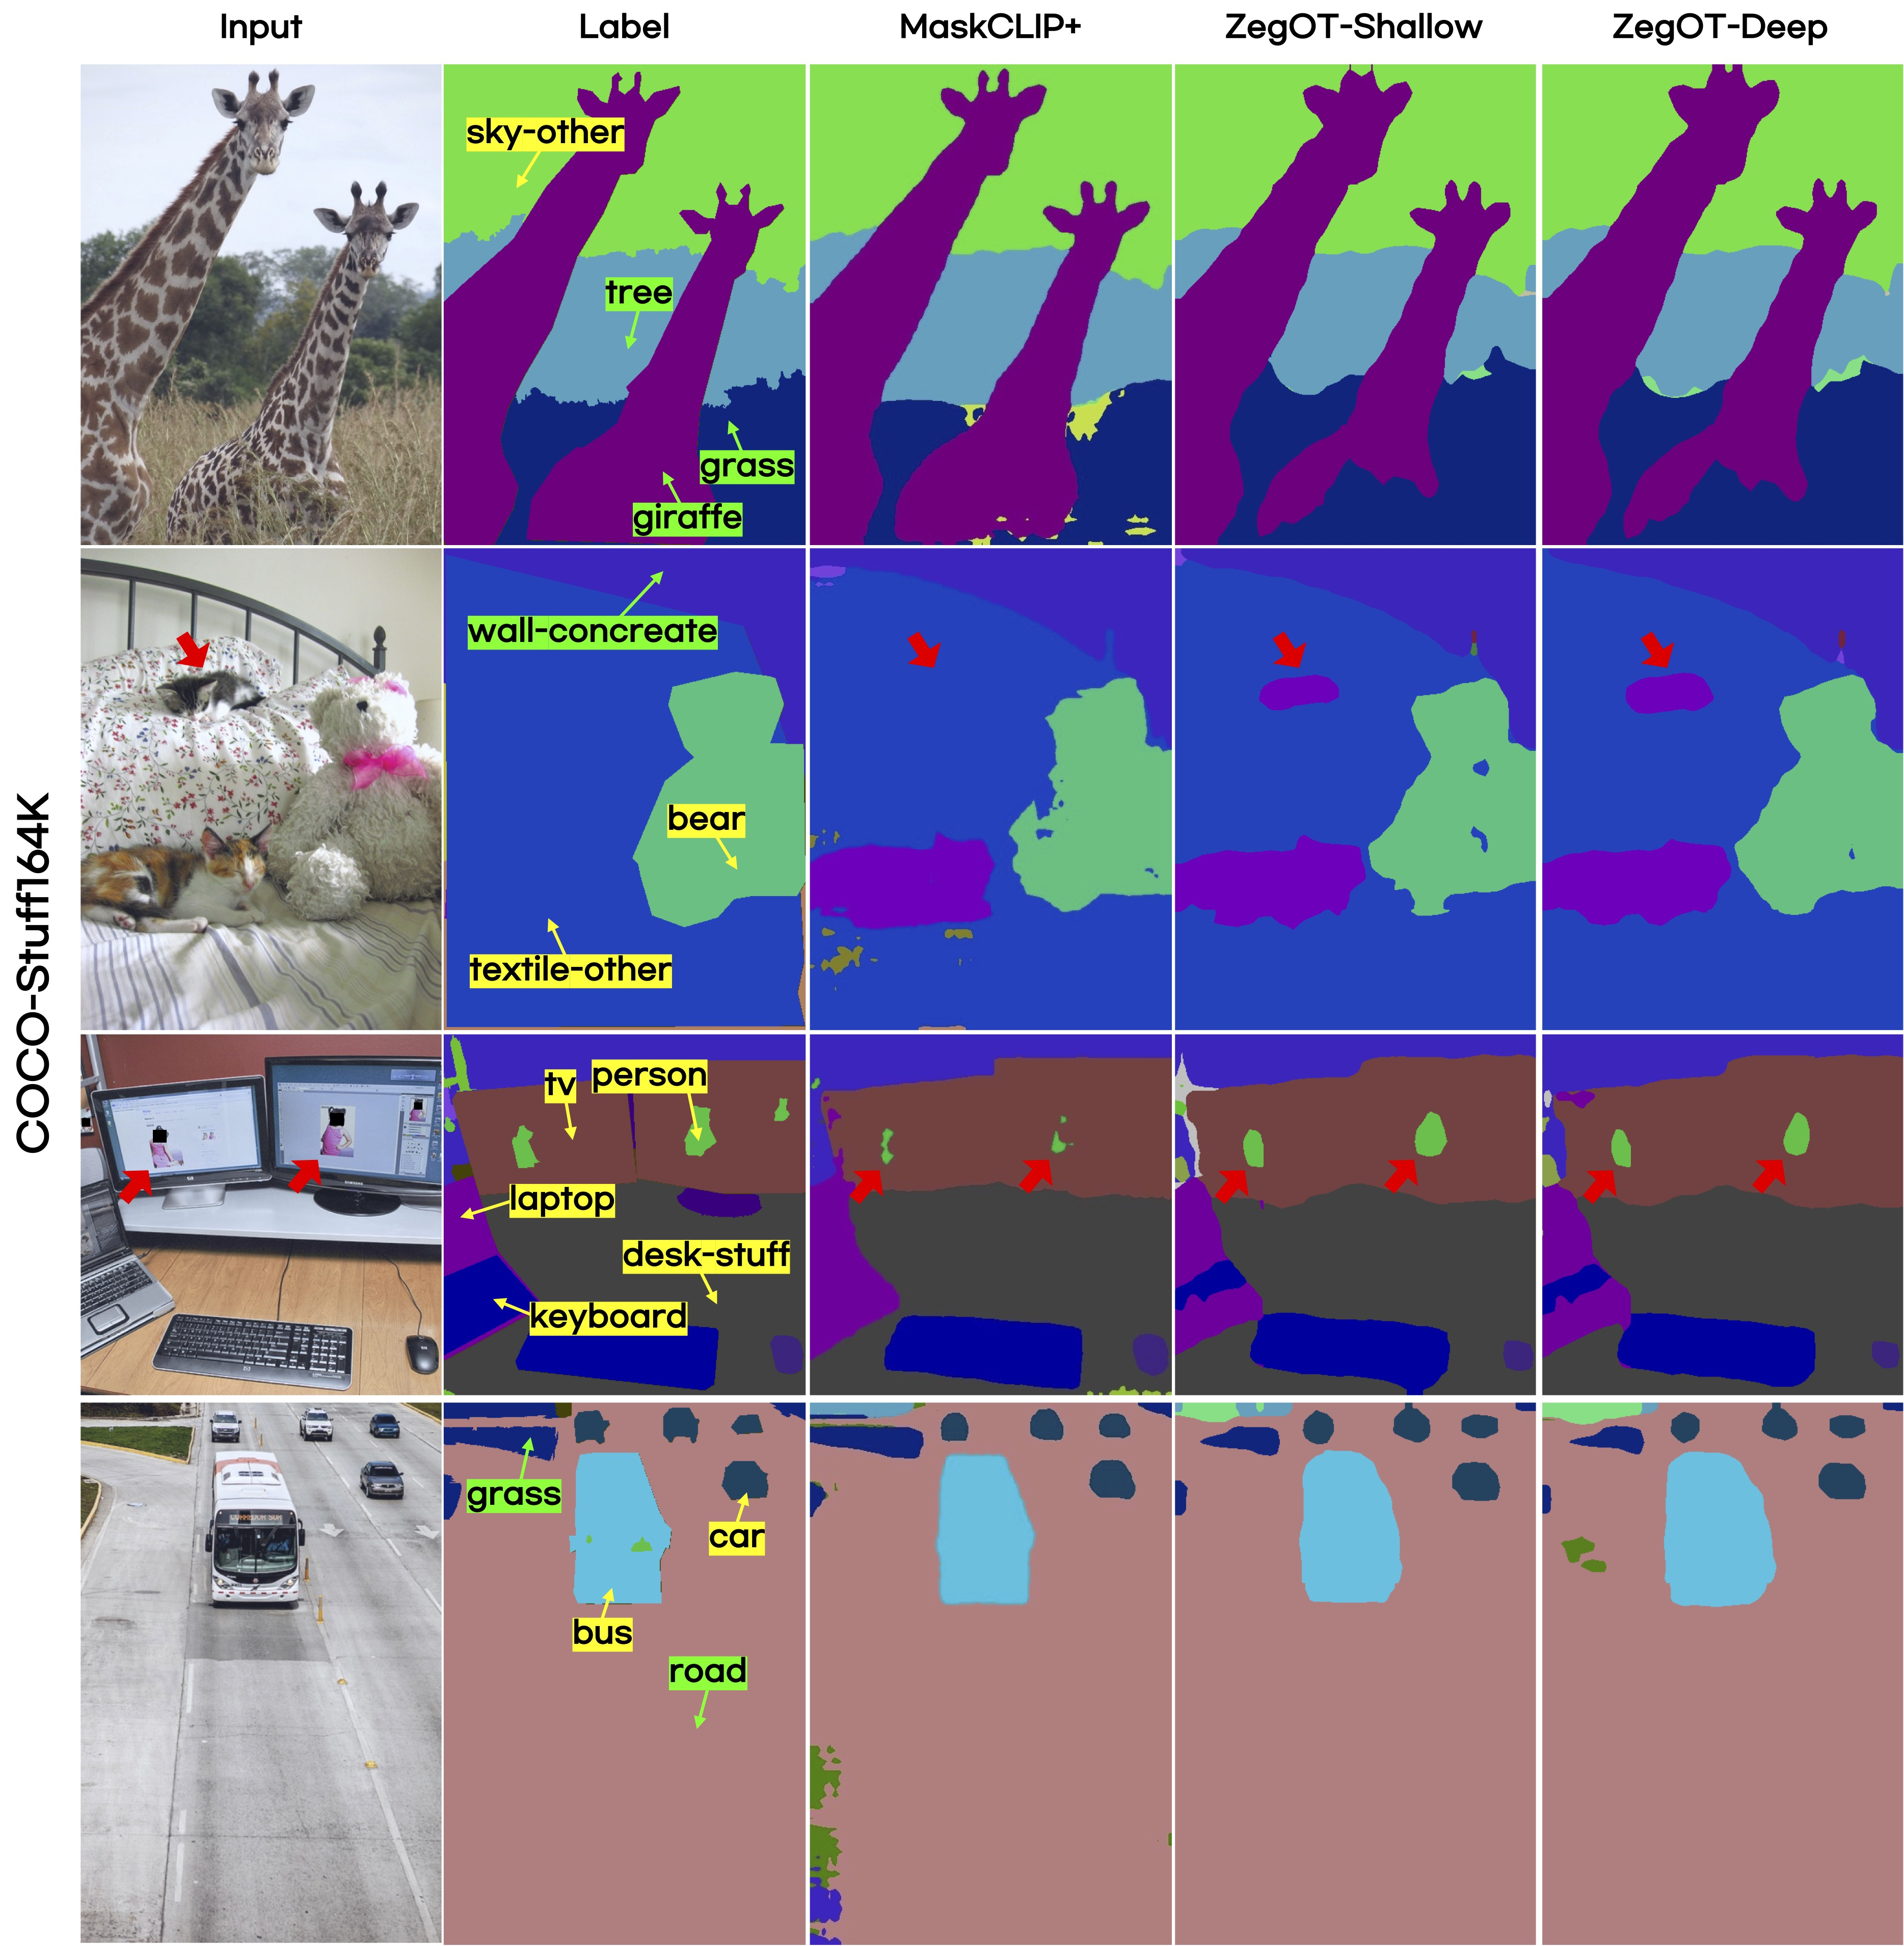
\includegraphics[width=0.97\linewidth]{fig/seg_appen.jpg}
\caption{Qualitative zero-shot segmentation results on COCO-Stuff164K dataset. The  \colorbox{yellow}{yellow} tag indicates seen classes, while the \colorbox{green}{green} tag indicates unseen classes. {Surprisingly, our ZegOT-Shallow and ZegOT-Deep effectively segment a tiny cat that does not even belong to the ground truth (see red arrows in 2nd row), and properly segment the person class within the small-sized portraits (see red arrows in 3rd row), while the previous SOTA method shows inferior performance on these features.} }
\label{fig_seg_appen}
\end{center}
\vskip -0.1in
\end{figure*}
%%%%%%%%%%%%%%%%%%%%%%%%%%%%%%%%%%%%%%%%%%%%%%%%%%%%%%%%%%%%%%%%%%%%%%%%%%%%%%%


%%%%%%%%%%%%%%%%%%%%%%%%%%%%%%%%%%%%%%%%%%%%%%%%%%%%%%%%%%%%%%%%%%%%%%%%%%%%%%%
%% Segmentation comparison COCO

\begin{figure*}[!t]
\vskip 0.1in
\begin{center}
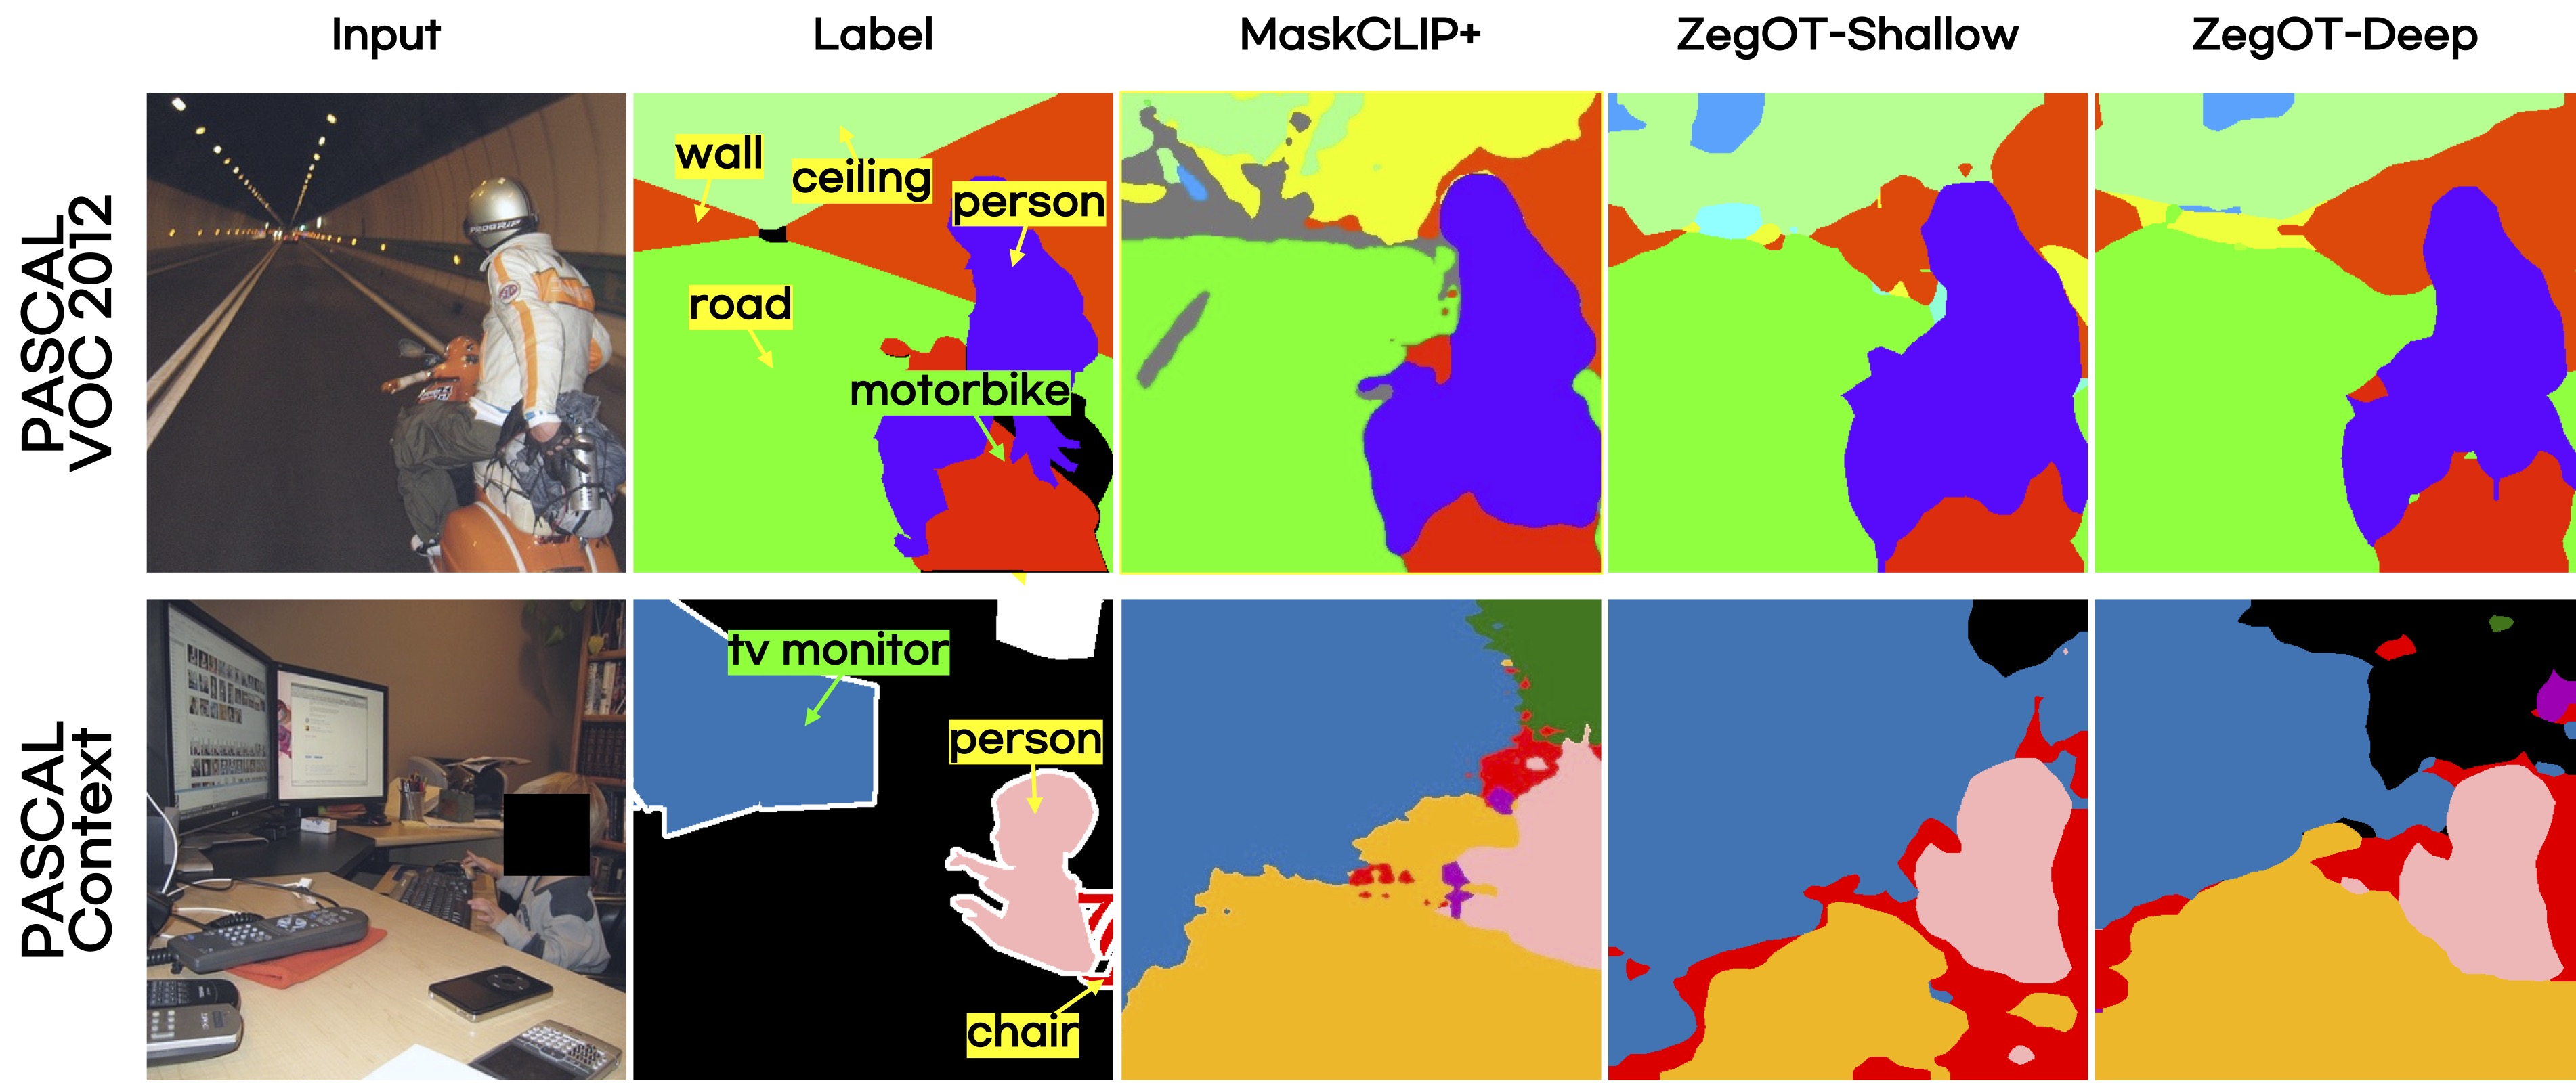
\includegraphics[width=0.97\linewidth]{fig/seg_appen2.jpg}
\caption{Qualitative zero-shot segmentation results on PASCAL VOC 2012 and PASCAL Context datasets. The  \colorbox{yellow}{yellow} tag indicates seen classes, while the \colorbox{green}{green} tag indicates unseen classes. }
\label{fig_seg_appen2}
\end{center}
\vskip -0.1in
\end{figure*}
%%%%%%%%%%%%%%%%%%%%%%%%%%%%%%%%%%%%%%%%%%%%%%%%%%%%%%%%%%%%%%%%%%%%%%%%%%%%%%%


%%%%%%%%%%%%%%%%%%%%%%%%%%%%%%%%%%%%%%%%%%%%%%%%%%%%%%%%%%%%%%%%%%%%%%%%%%%%%%%
%% Appendix Result Figure

\begin{figure*}[!h]
\vskip 0.1in
\begin{center}
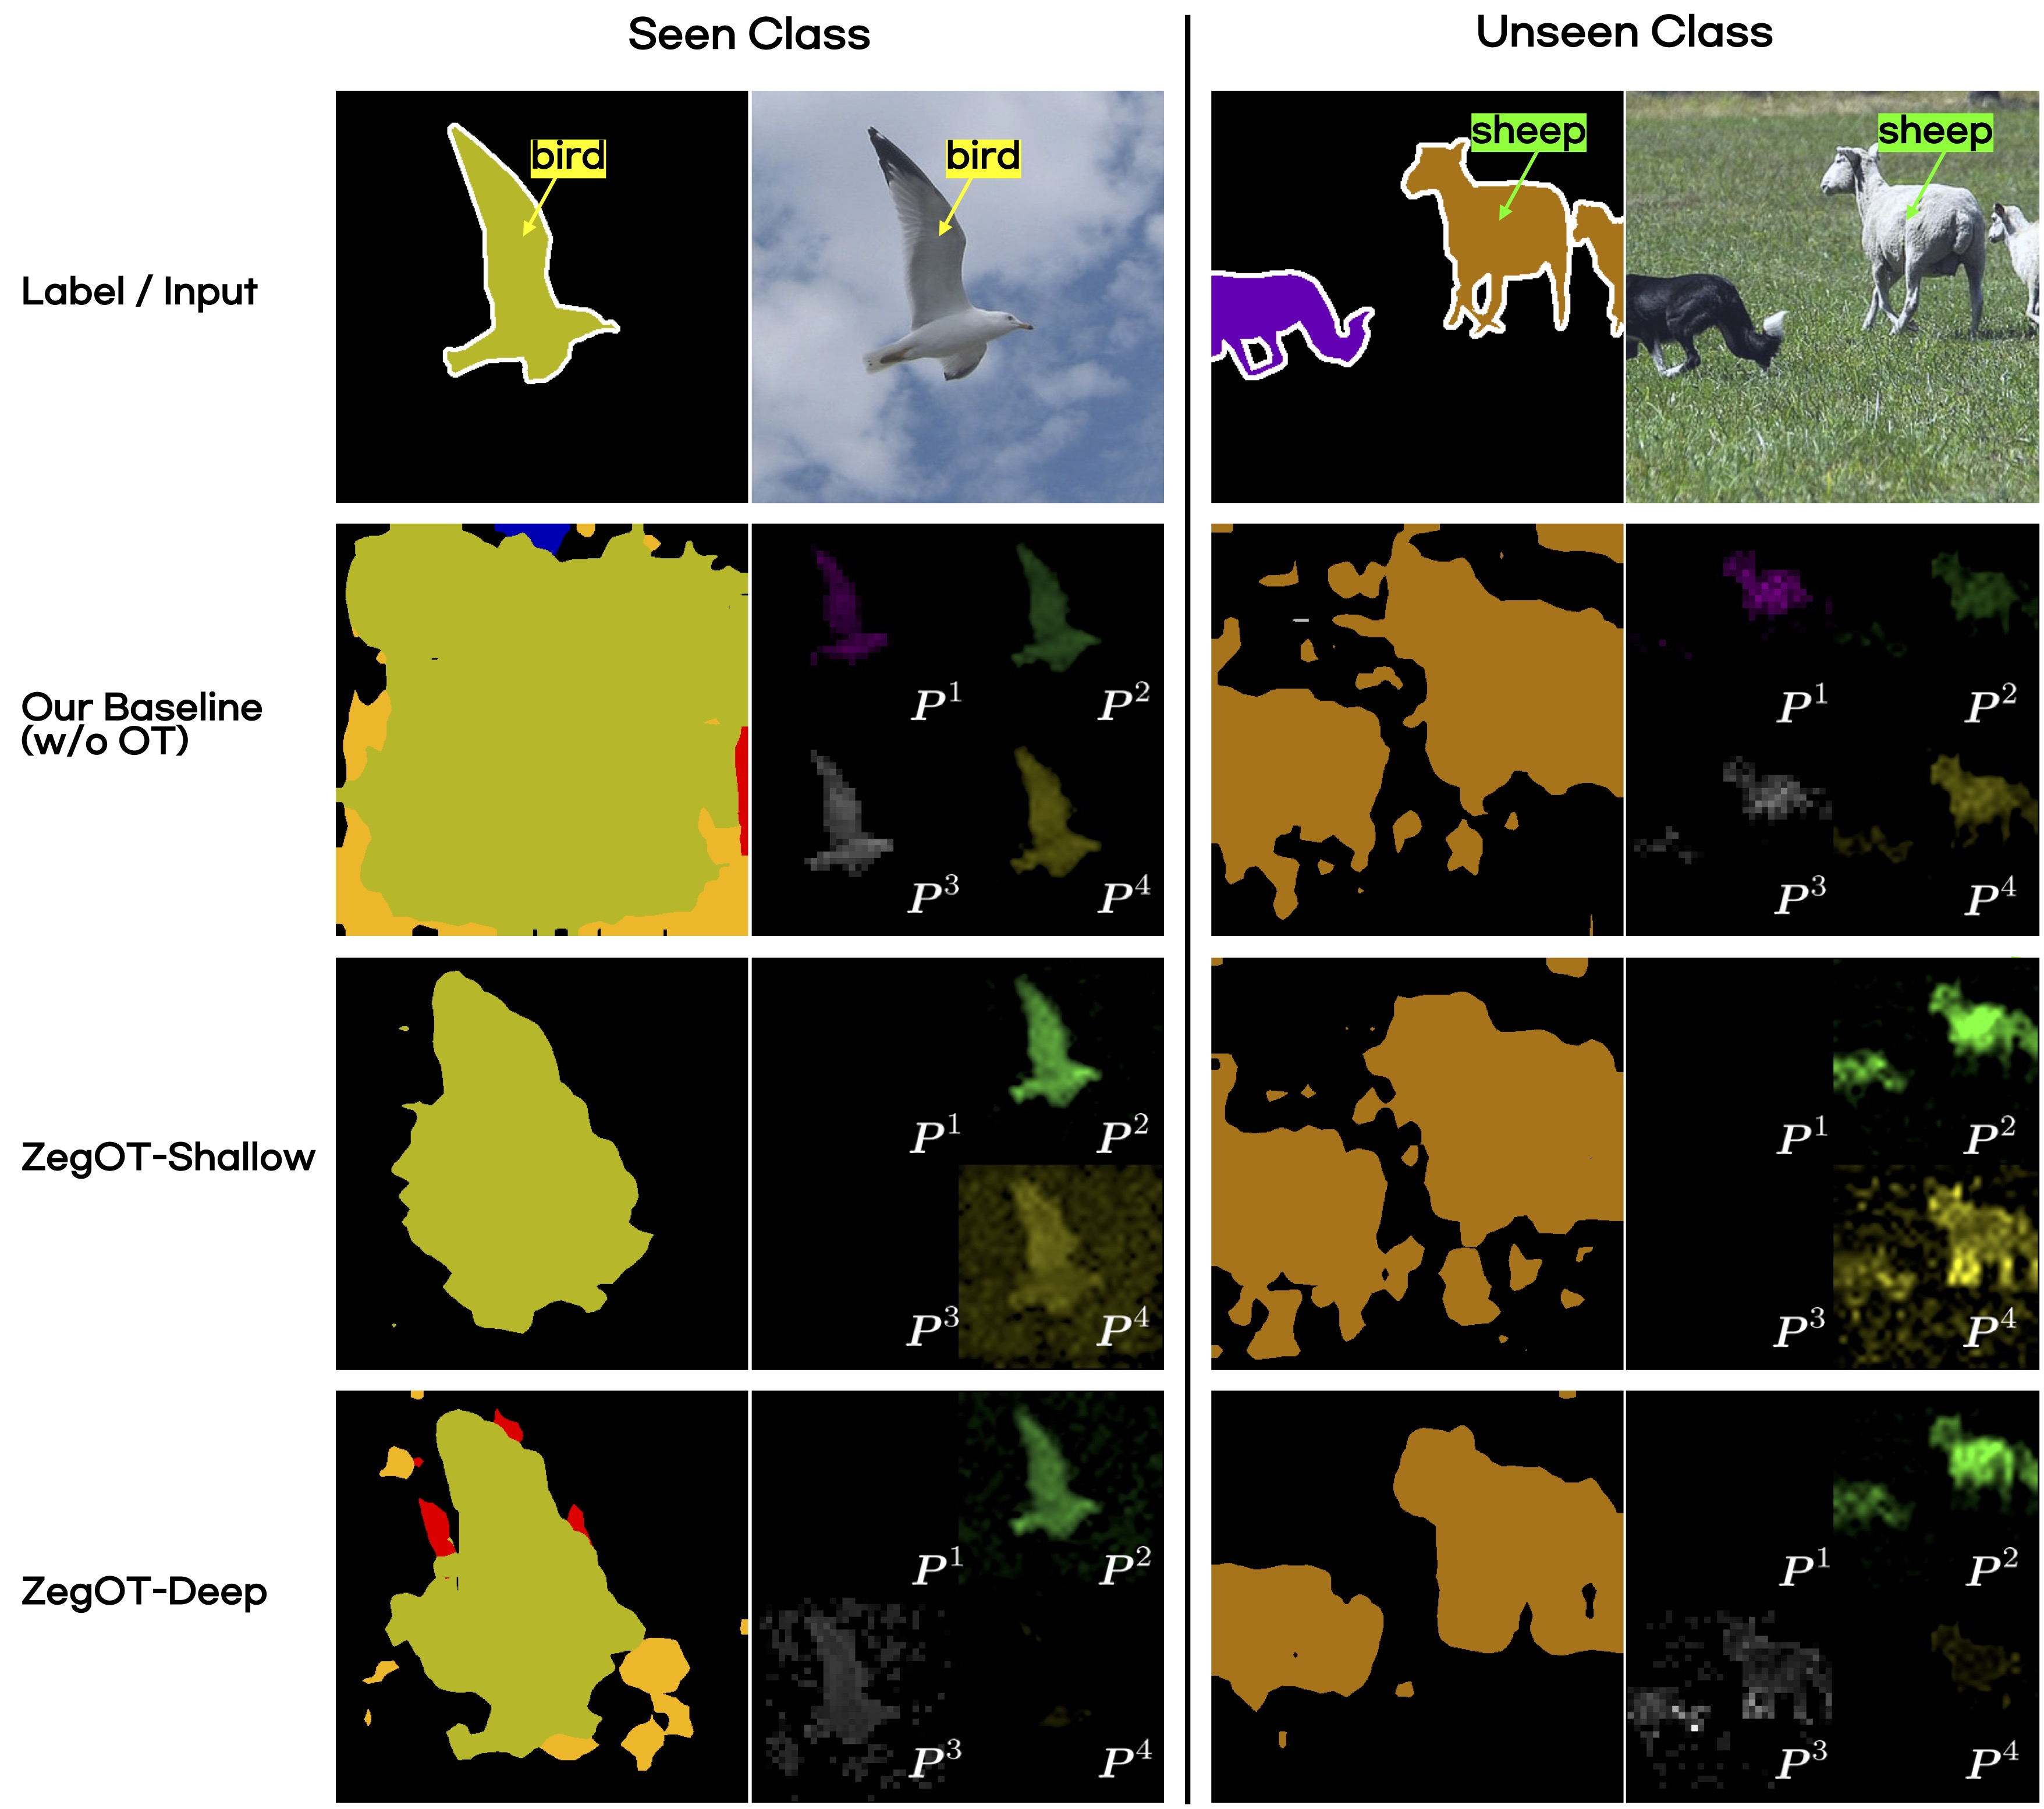
\includegraphics[width=1\linewidth]{fig/scoremap_apen.jpg}
\caption{Visualization of the learned text prompt and image pixel alignment. The \colorbox{yellow}{yellow} tag indicates seen classes, while the \colorbox{green}{green} tag indicates unseen classes. For each method, we present its segmentation result (left) and $N$ multiple text prompts-related score matrix activated by the predicted class (right). 
In the baseline method without OT, all the $\bs{P}^i$-related score matrices resemble each others. On the other hand, our ZegOT-Shallow and ZegOT-Deep show separate score matrices, with ZegOT-Deep more focusing on different semantic attributes of the predicted class object.
}
\label{fig_score_appen}
\end{center}
\vskip -0.1in
\end{figure*}
%%%%%%%%%%%%%%%%%%%%%%%%%%%%%%%%%%%%%%%%%%%%%%%%%%%%%%%%%%%%%%%%%%%%%%%%%%%%%%%




\end{document}
